
\documentclass[a4paper]{article}
\usepackage{pslatex}
\usepackage[T1]{fontenc}
\usepackage[utf8x]{inputenc}
\setlength\parskip{\medskipamount}
\setlength\parindent{0pt}
\usepackage{graphicx}
\usepackage{amssymb}
%\usepackage{hyperref}

\makeatletter

\providecommand{\boldsymbol}[1]{\mbox{\boldmath $#1$}}
\newcommand{\ASL}			{ASL}
\newcommand{\OSC}[1]		{\texttt{#1}}
\newcommand{\lra}			{$\leftrightarrow$}
\newcommand{\seg}[1]		{Seg(#1)}

\setlength{\parskip}{1mm}

\makeatother

\begin{document}

\title{FaustLive - Control/Compute/Communicate \\ All The Possibilities\\ v.2.0}

\author{Grame, Centre National de Création Musicale\\
{\small <research@grame.fr>} \\
\vspace{2mm}
[ANR-12-CORD- 0009] and [ANR-13-BS02-0008]
}

\maketitle

\topskip0pt

\vspace{\fill}

\vspace{\fill}
%==================================================================================================
\newpage
\tableofcontents

\newpage
\section{The Control-Compute-Communicate Model}

 We can roughly describe any audio application as having three principal parts (see Figure {\ref{fig:structure}}), which are named with the  {\it Control-Compute-Communicate}  terminology:

\begin{itemize}

\item {\it control}: the control part changes the parameters in real-time  

\item  {\it compute}: the audio DSP computation processes audio inputs and produces audio outputs  

\item {\it communicate}   (with the audio card):  the audio rendering part triggers the audio computation.  

\end{itemize}

\begin{figure}[!ht]
\begin{center}
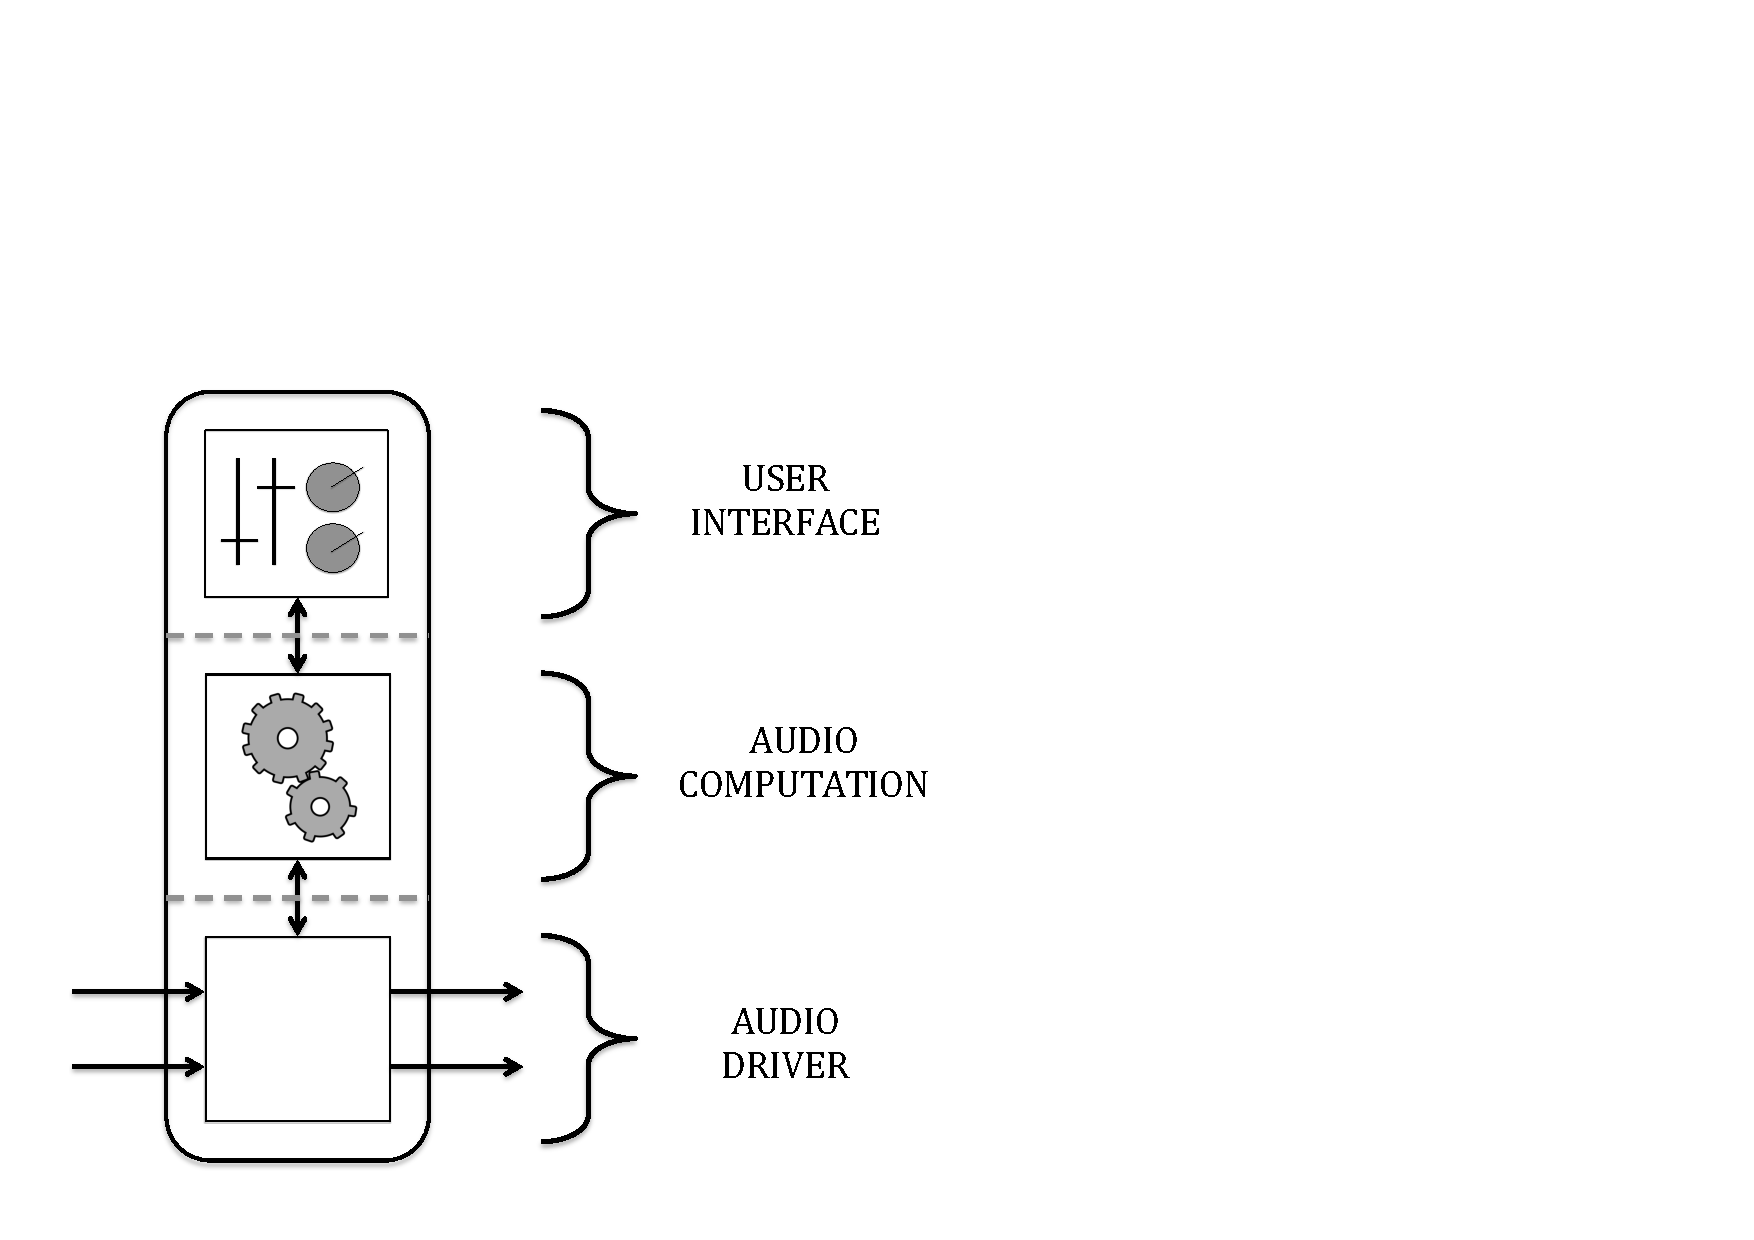
\includegraphics[width=0.75\columnwidth]{images/2-Faust_Construction}
\caption{Audio application structure}
\label{fig:structure}
\end{center}
\end{figure}

For further information about this model and some implementations : \cite{CCC} and \cite{FaustLive} 


\bibliographystyle{plain}
\bibliography{RemoteFeatures}

\newpage
\section{Constraints}\label{constraints}

The main difficulty is to think through the interactions of every feature:
\begin{itemize}
\item local/remote processing
\item remote control (OSC, HTTP, NetJack)
\item remote rendering (NetJack)
\end{itemize}

For each feature, the compilation chain has to be  make sure we have the exact same behavior (compilation, synchronization of params/edition, crossfade, session saving/recall, etc). \\

For now, it is possible to use the remote processing or the publish feature but it was never validated that every thing works together. \\

Moreover, FaustLive was created as a pile of features that were more or less independent. This is why FaustLive can have multiple servers running : 1 for each HTTP interface + 1 to center all HTTP interfaces + 1 for remote processing + etc

There might be a way to simplify this. 

\newpage
\section{All the use cases}

%%%%%%%%%%%%%%MAIN CONFIG%%%%%%%%%%%%%%%%%
\subsection{FaustLive Main Use}
This is the usual configuration for any Faust application, whether it is a standalone application, a plugin or running in FaustLive.
\begin{figure}[!h]
\begin{center}
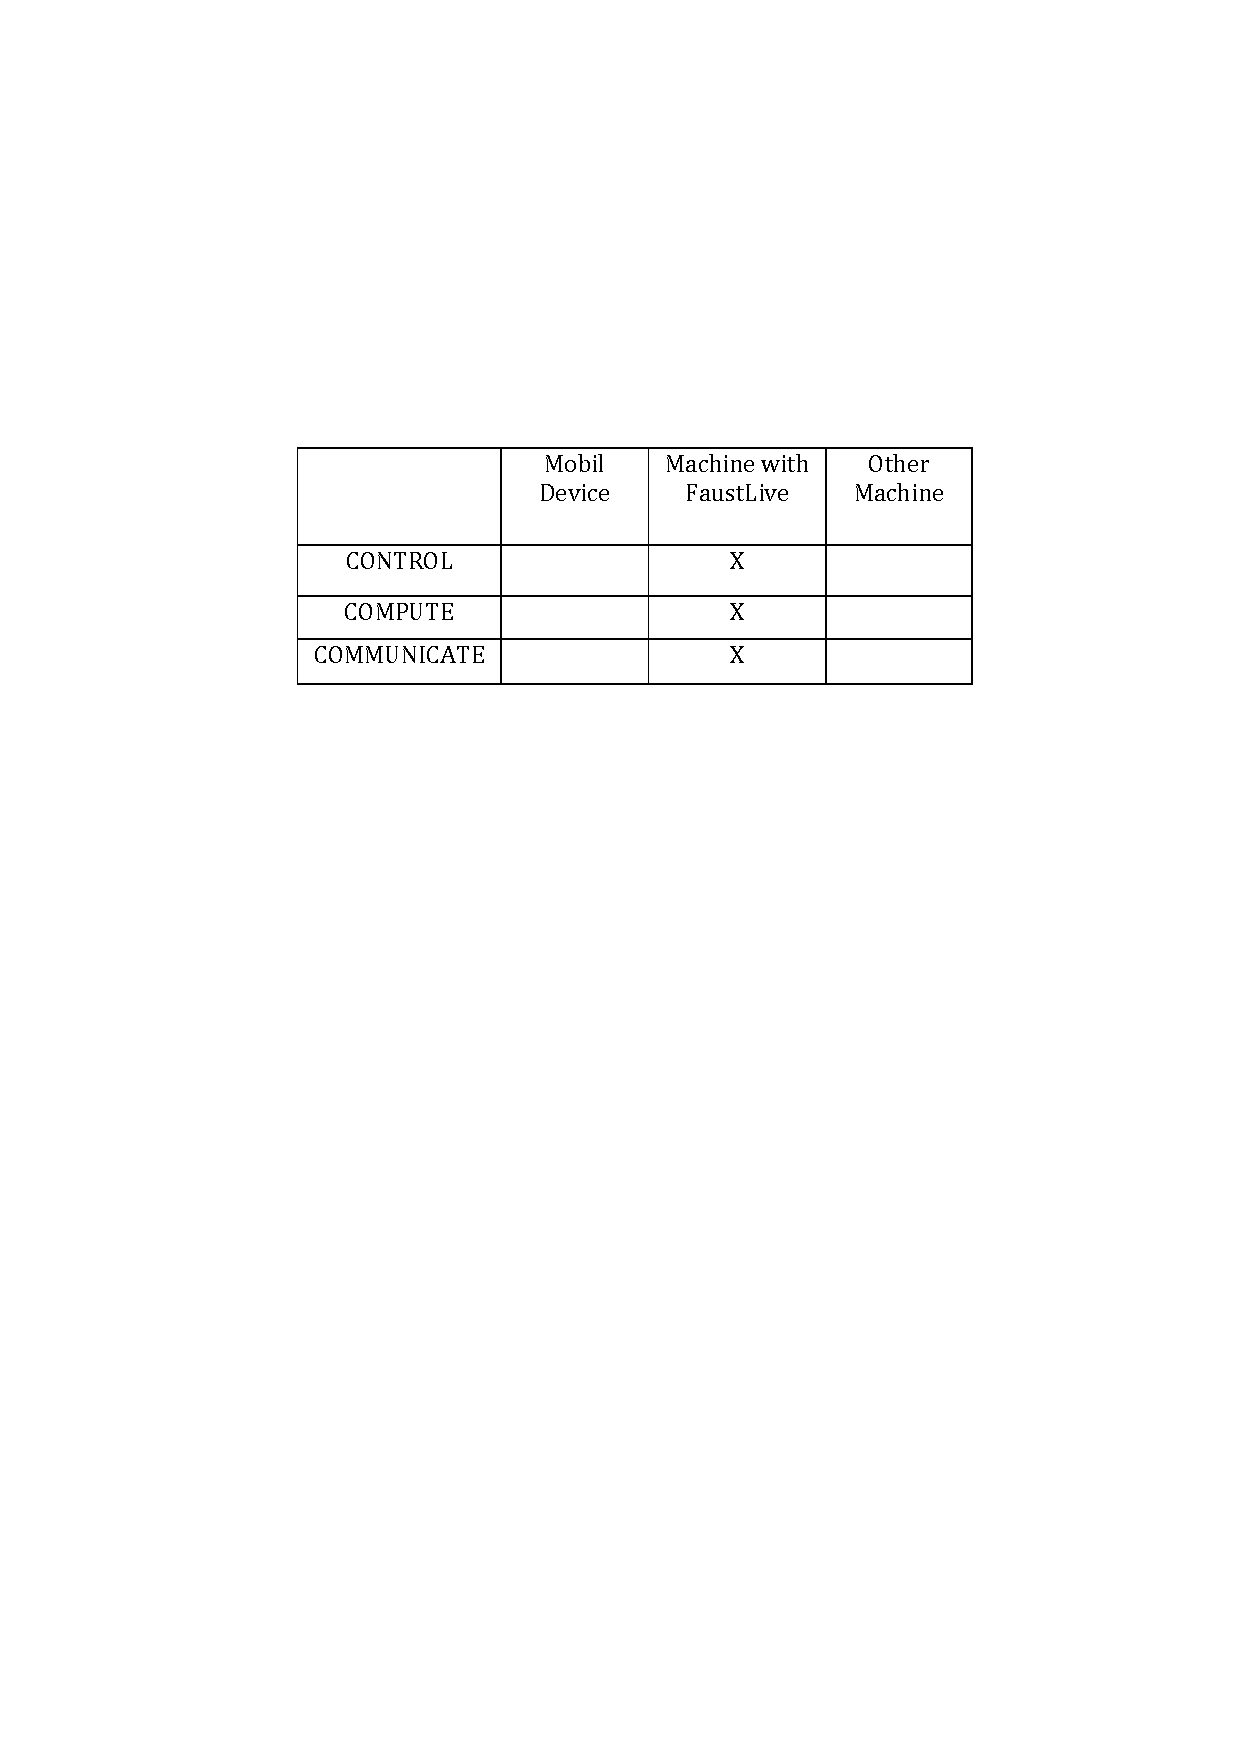
\includegraphics[width=0.7\columnwidth]{images/1CCC}
\caption{Control-Compute-Communicate Division for the main uses of FaustLive}
\label{fig:1CCC}
\end{center}
\end{figure}

\begin{figure}[!h]
\begin{center}
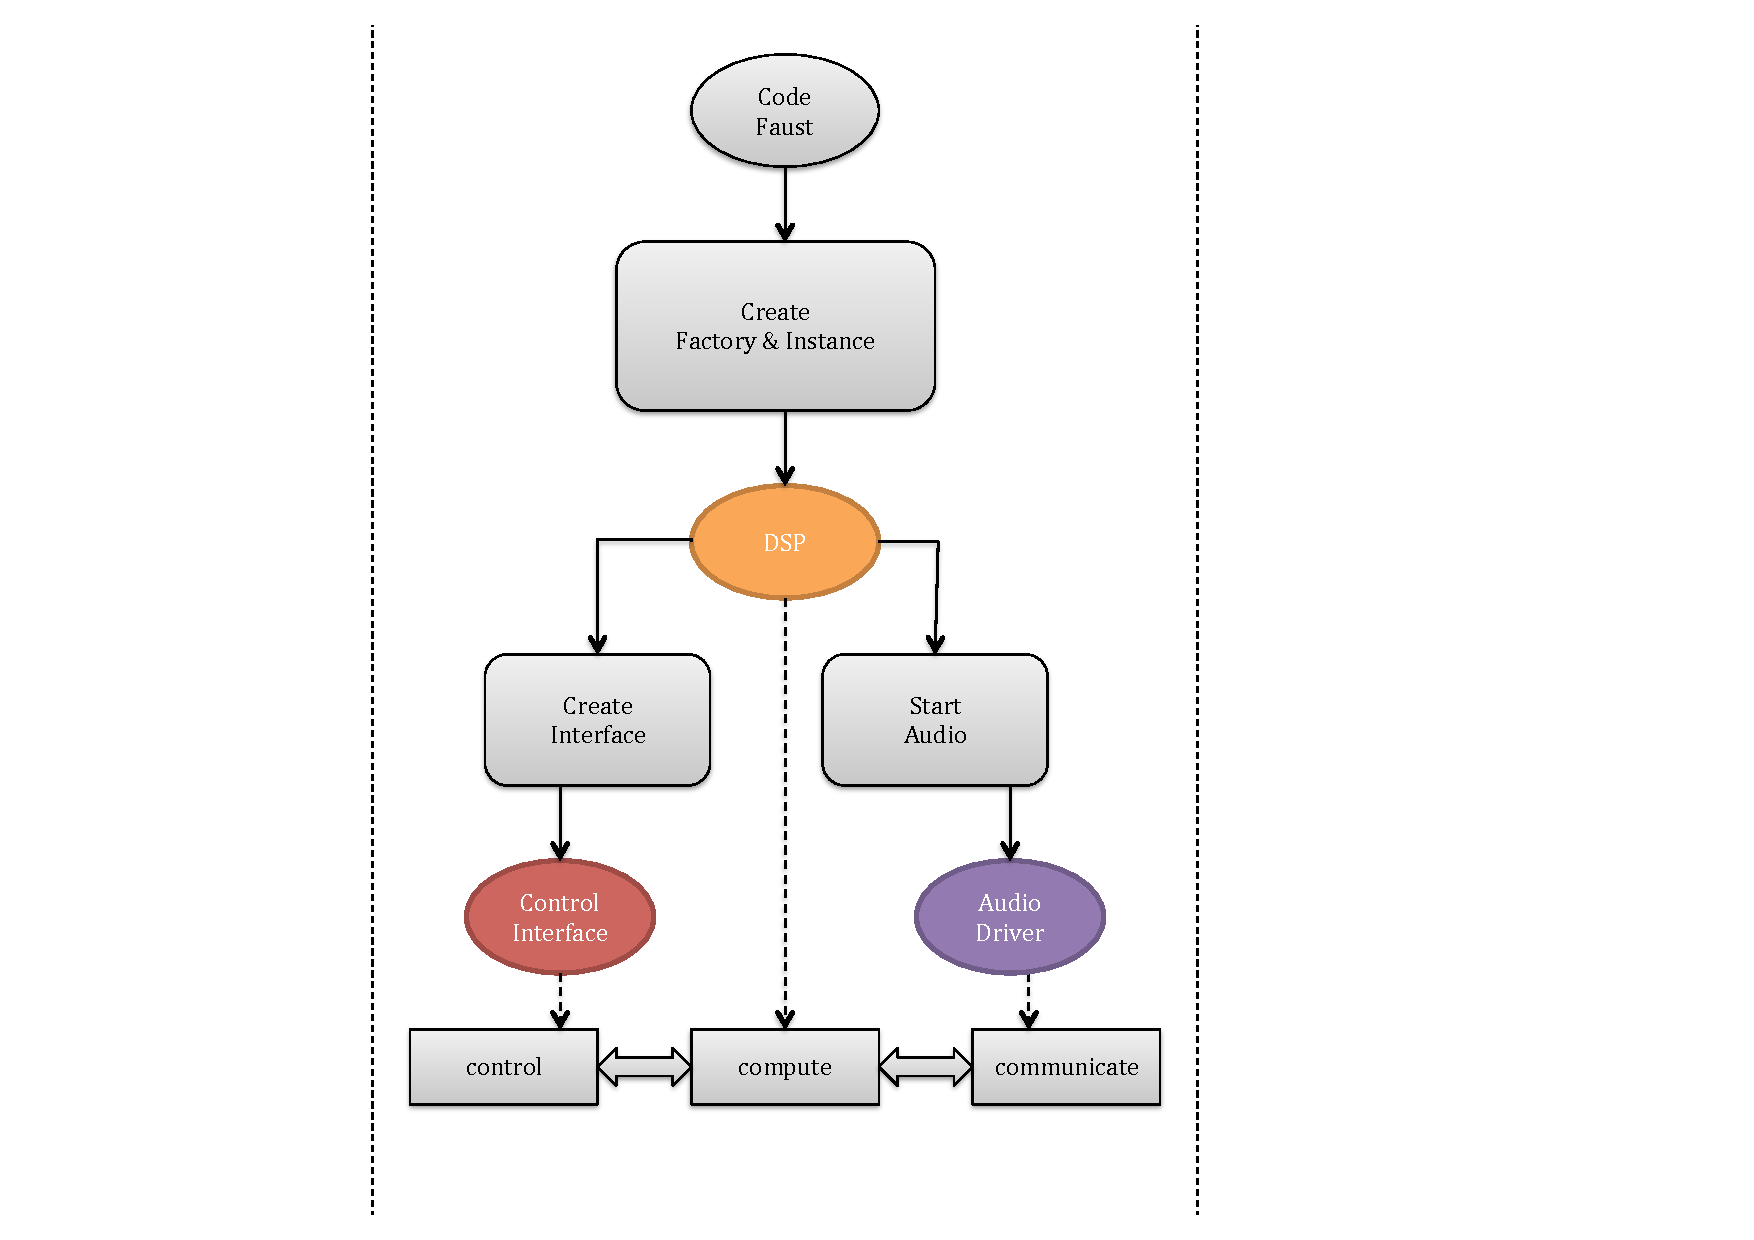
\includegraphics[width=\columnwidth]{images/CCC1}
\caption{Creation of the Interface/DSP/Driver for the main uses of FaustLive}
\label{fig:CCC1}
\end{center}
\end{figure}

%%%%%%%%%%%%%%REMOTE CONTROL%%%%%%%%%%%%%%%%%
\newpage
\subsection{ Using the remote control (OSC, HTTP or other?)} \label{remotecontrol}
FaustLive creates an interface OSC or HTTP which means launching a server that waits for remote interfaces to synchronize. \\
From the remote device, we can then create the corresponding interface.\\

An idea implemented for HTTP remote interfaces but not OSC:
\begin{itemize}
\item The mobile device sends code to create the factory then gets back the interface while the processing and rendering are done in FaustLive. \\
A global server for HTTP handles all the declared HTTP interfaces. It can be interrogated to know all the available interfaces.
\end{itemize}

\begin{figure}[!h]
\begin{center}
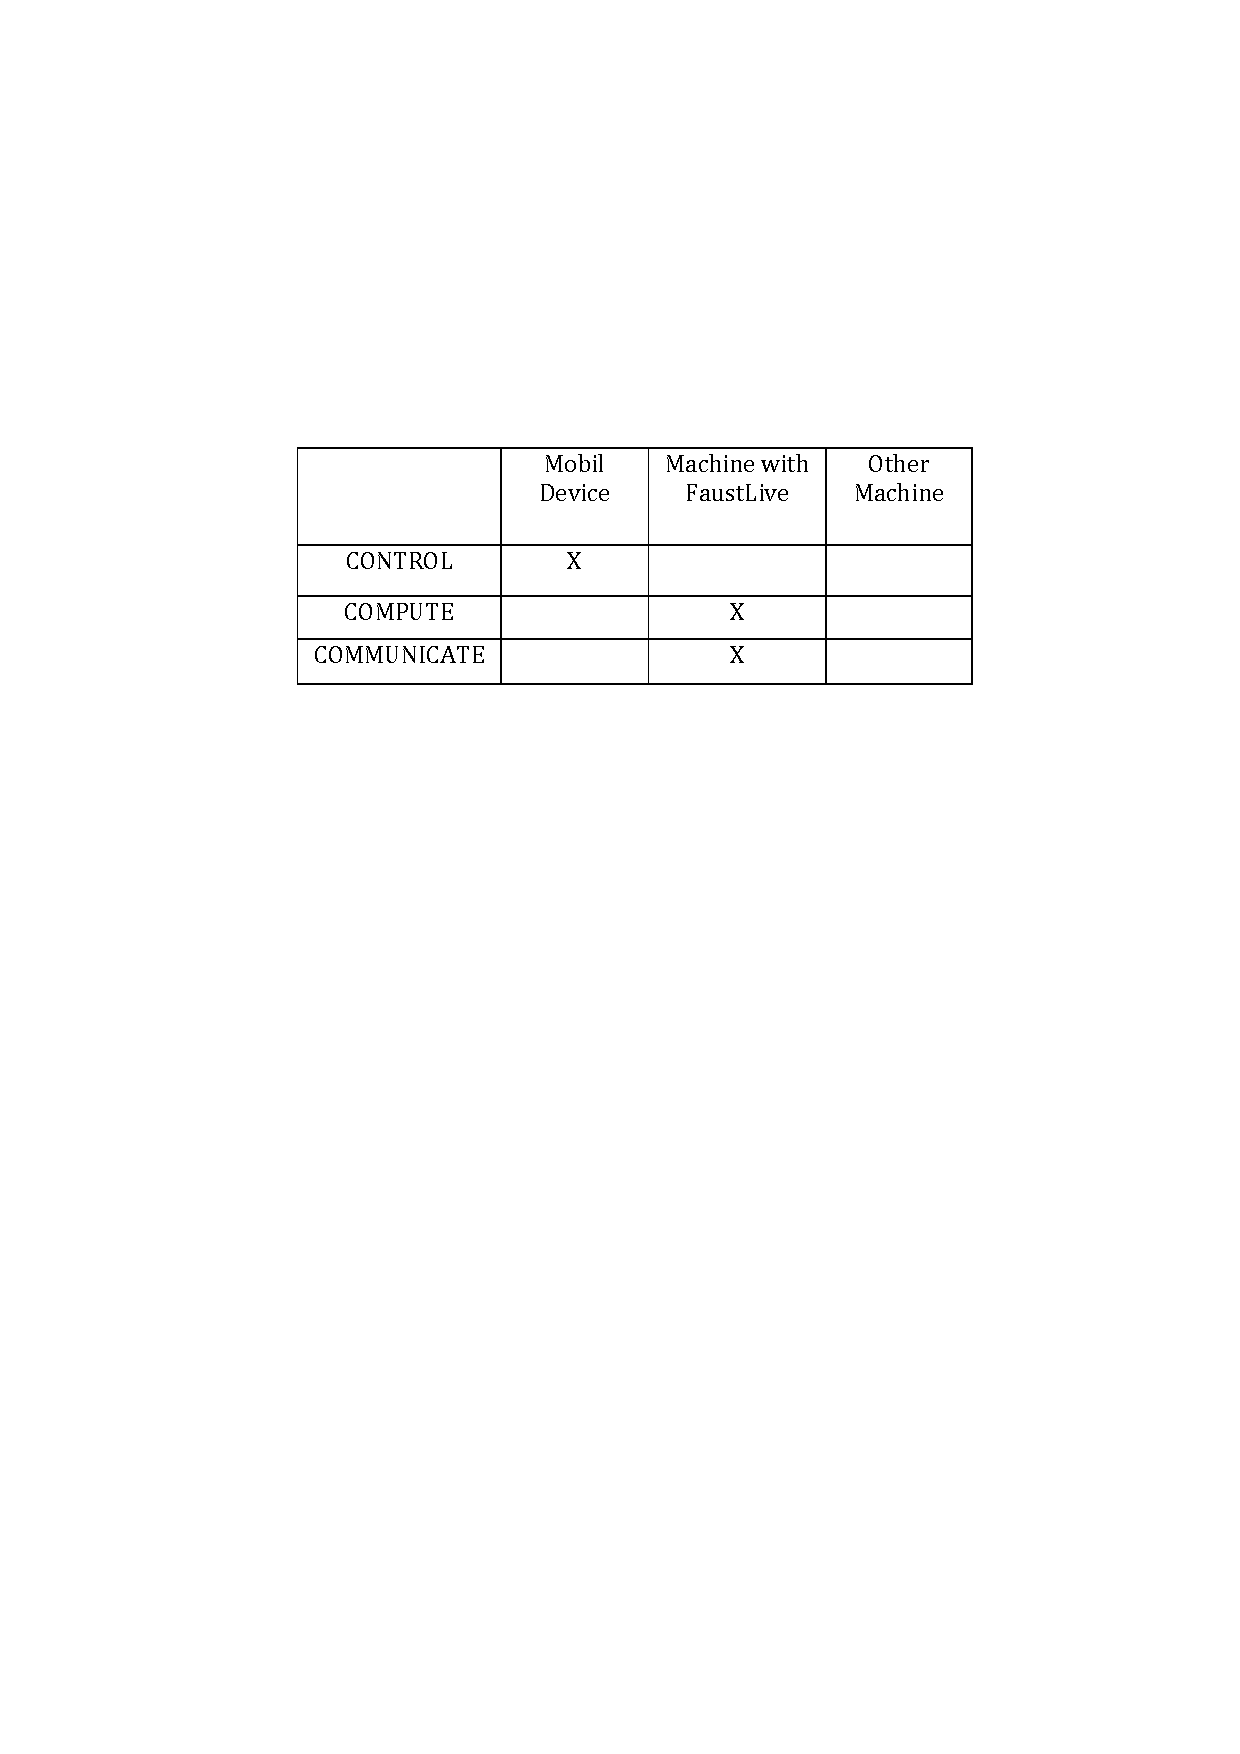
\includegraphics[width=0.7\columnwidth]{images/2CCC}
\caption{Control-Compute-Communicate Division with remote interface}
\label{fig:2CCC}
\end{center}
\end{figure}
\begin{figure}[!h]
\begin{center}
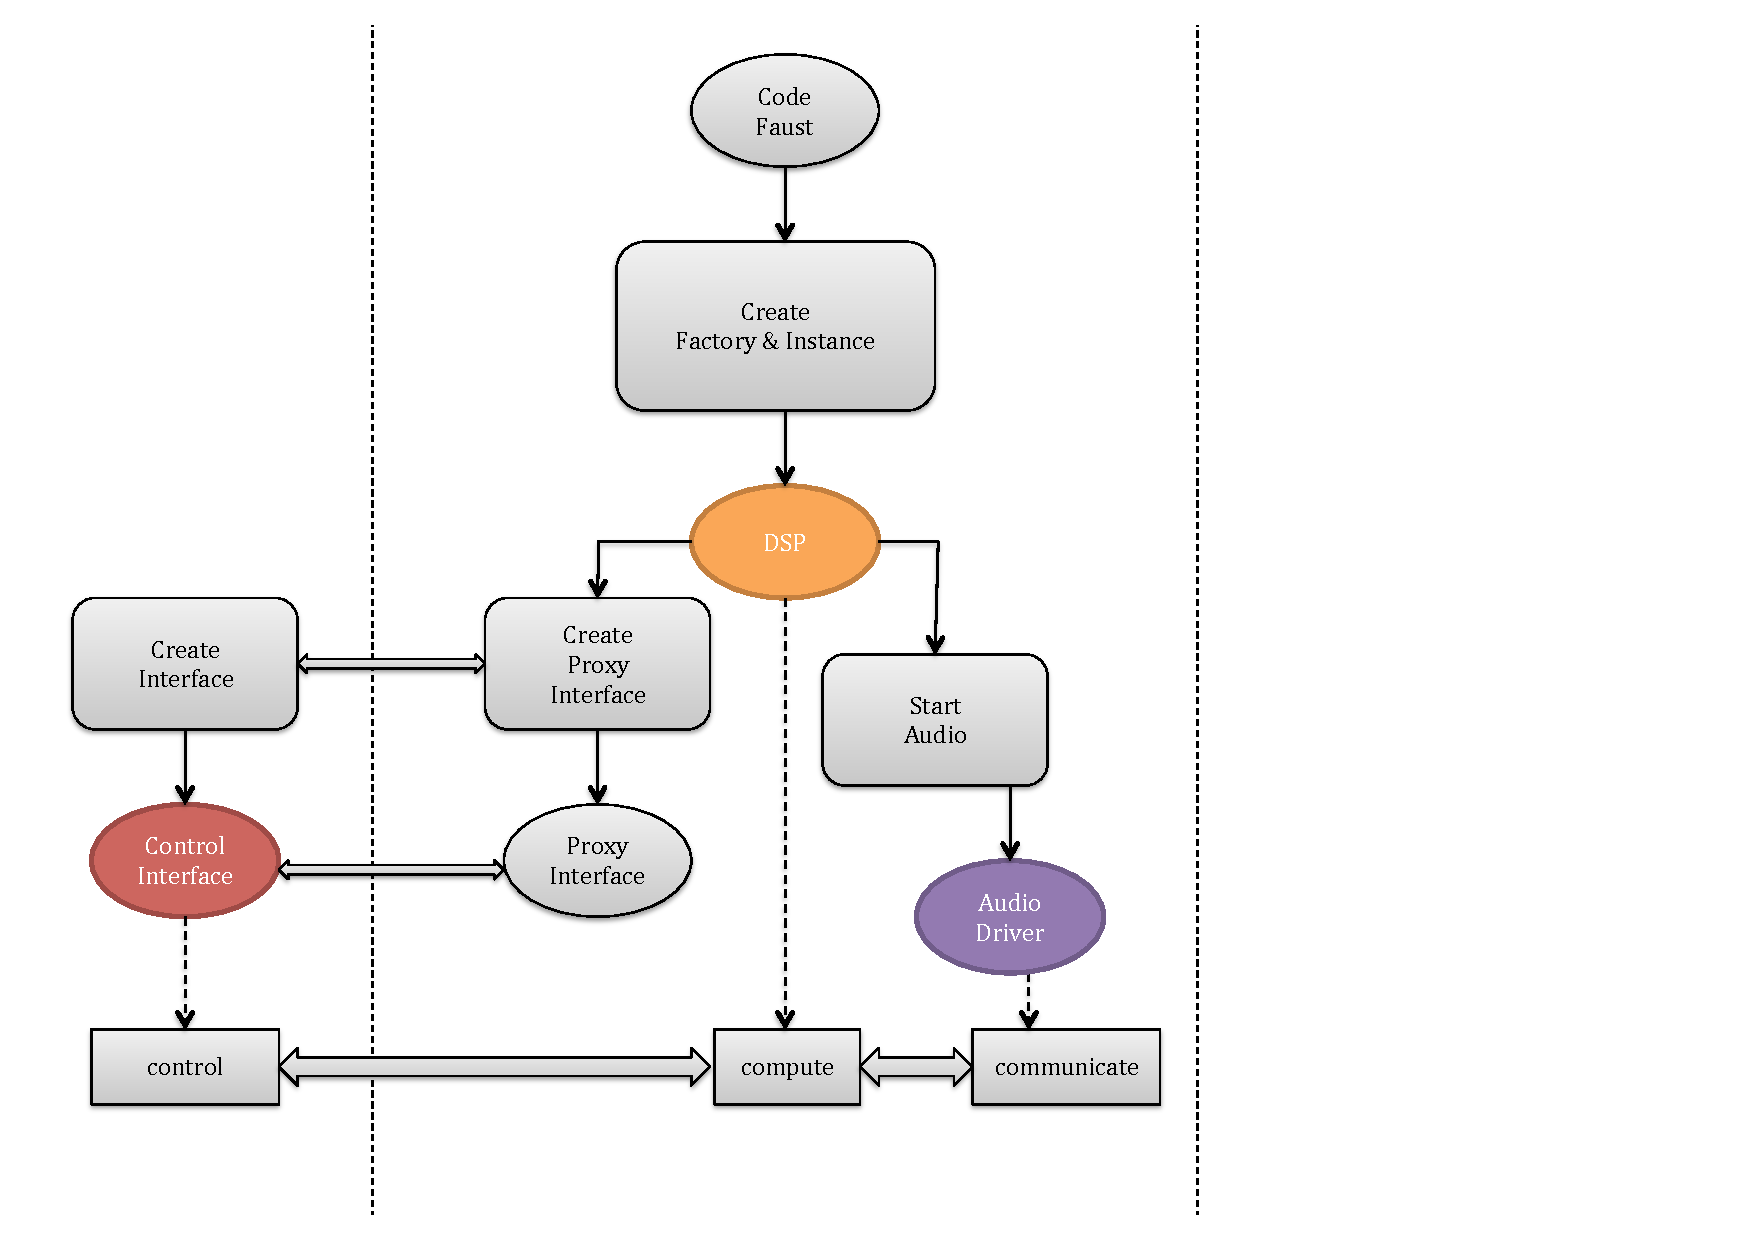
\includegraphics[width=\columnwidth]{images/CCC2}
\caption{Creation of the Interface/DSP/Driver for a remote control use case}
\label{fig:CCC2}
\end{center}
\end{figure}


%%%%%%%%%%%%%%REMOTE RENDER%%%%%%%%%%%%%%%%%
\newpage
\subsection {Using NetJack for remote audio rendering} \label{remoterendering}

In FaustLive, switch to NetJack as audio driver in the general preferences. 
\begin{figure}[!h]
\begin{center}
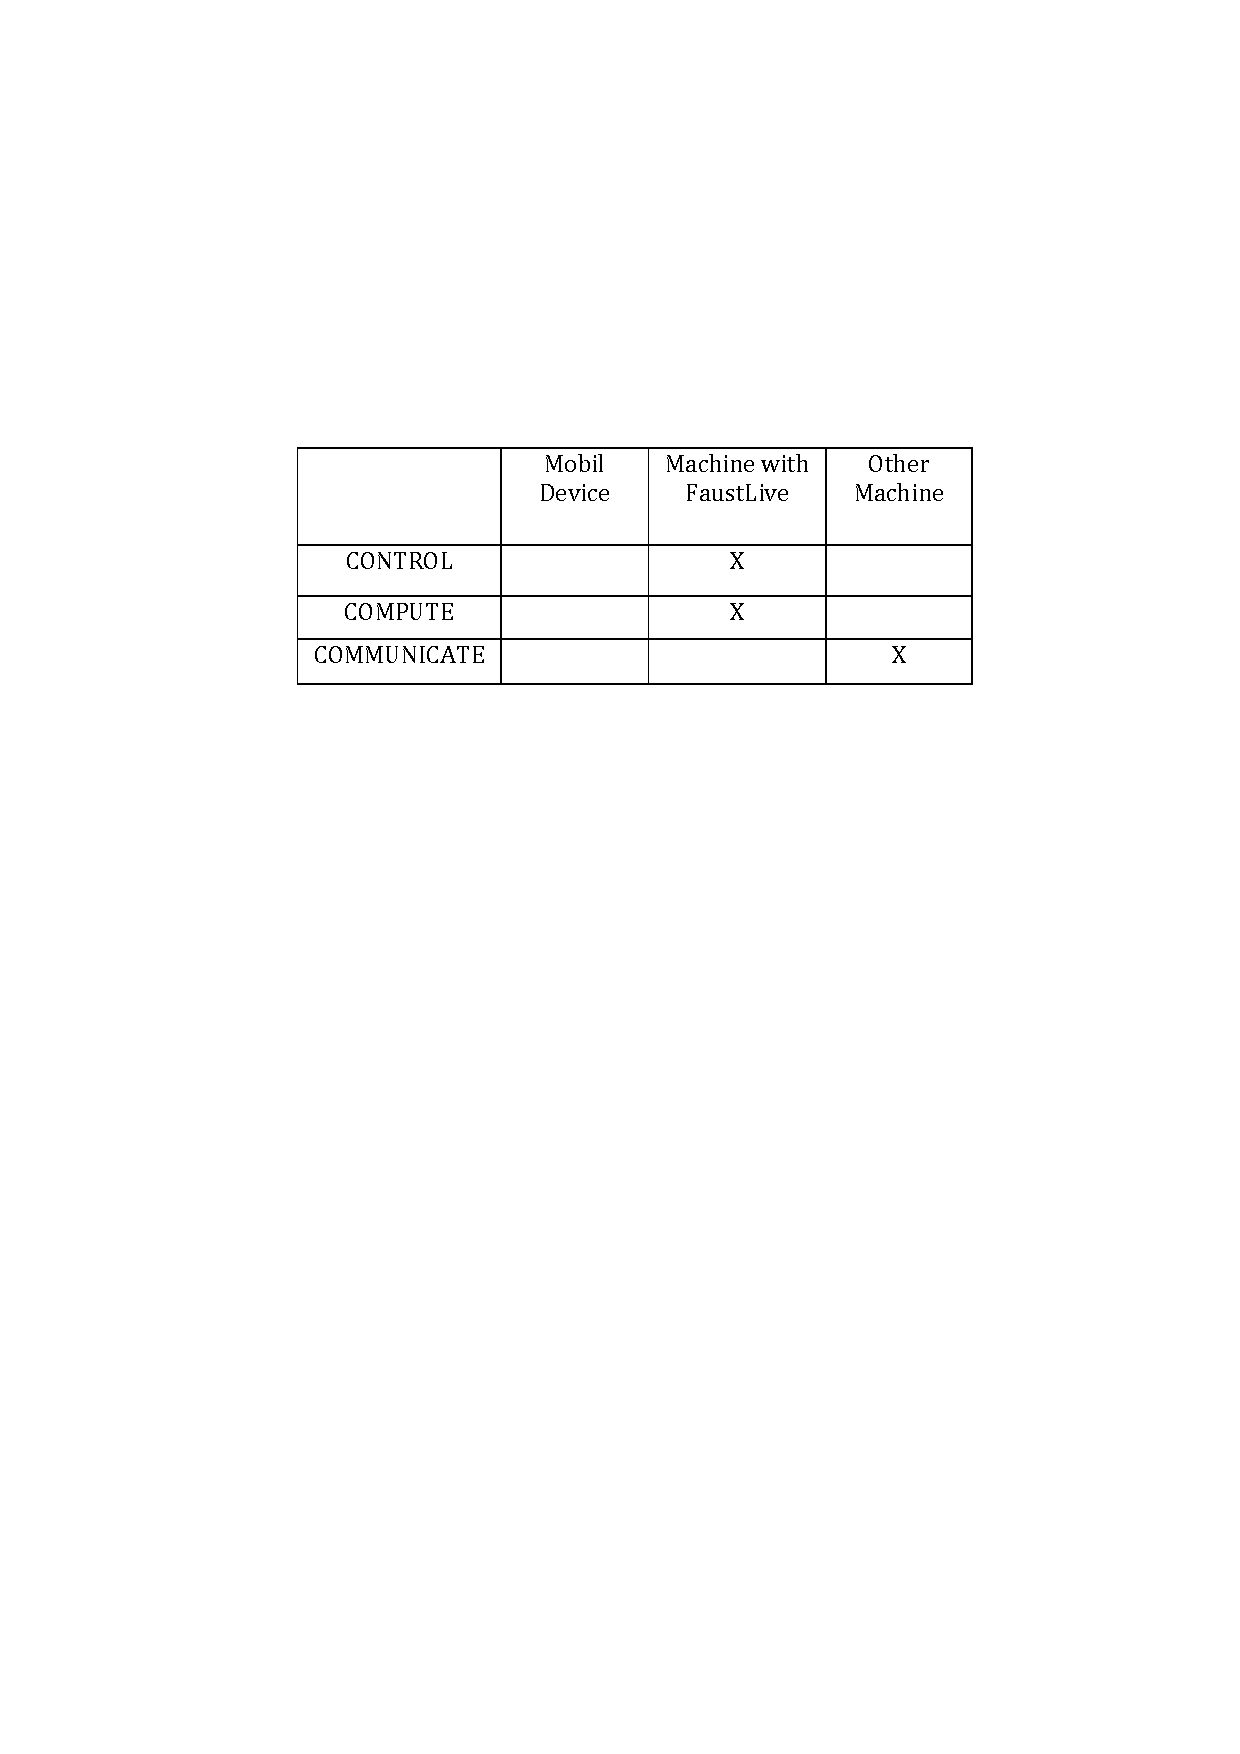
\includegraphics[width=0.7\columnwidth]{images/3CCC}
\caption{Control-Compute-Communicate Division with remote audio rendering}
\label{fig:3CCC}
\end{center}
\end{figure}
\begin{figure}[!h]
\begin{center}
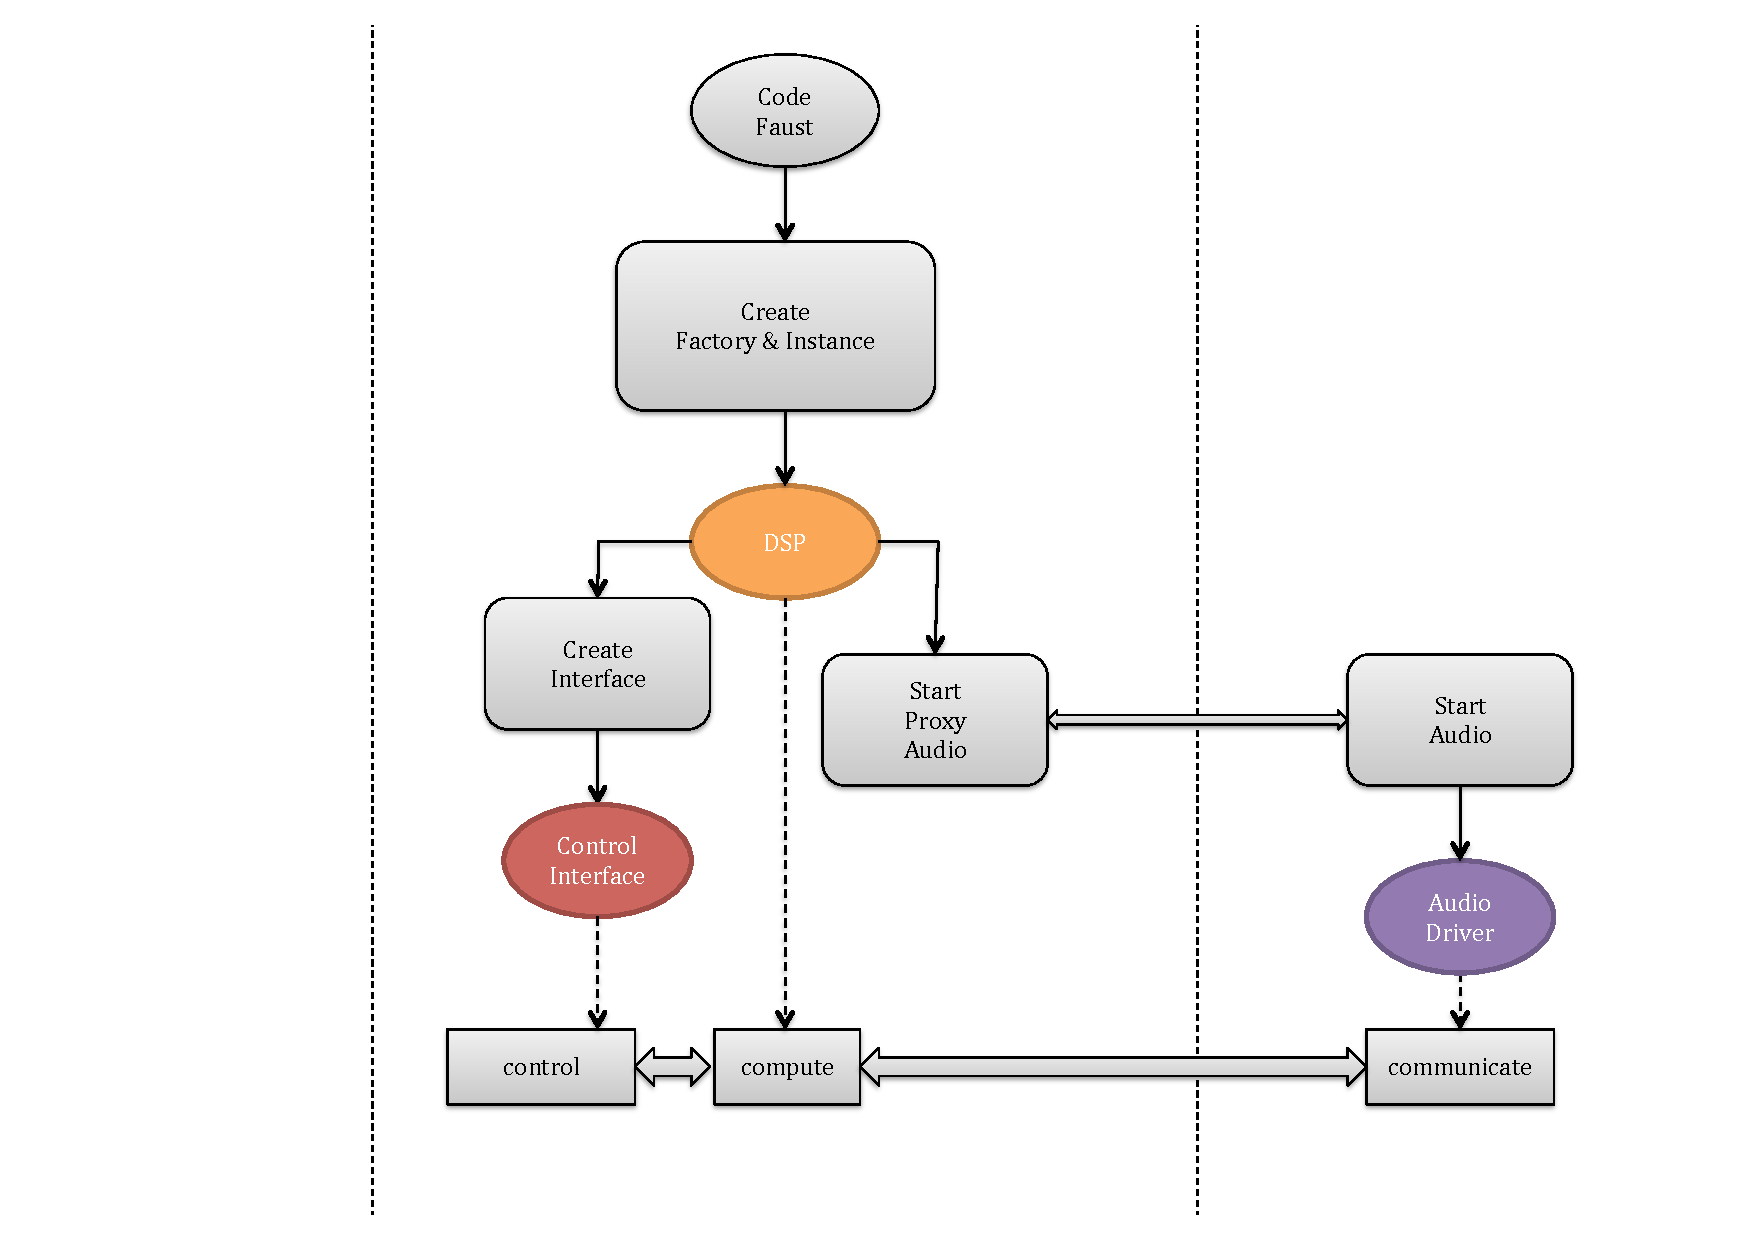
\includegraphics[width=\columnwidth]{images/CCC3}
\caption{Creation of the Interface/DSP/Driver for a remote rendering use case}
\label{fig:CCC2}
\end{center}
\end{figure}
%%%%%%%%%%%%%%REMOTE CONTROL & RENDER%%%%%%%%%%%%%%%%%
\newpage
\subsection{ Remote control and remote rendering}

Combining use case {\ref{remotecontrol}} and use case {\ref{remoterendering}}.

\begin{figure}[!h]
\begin{center}
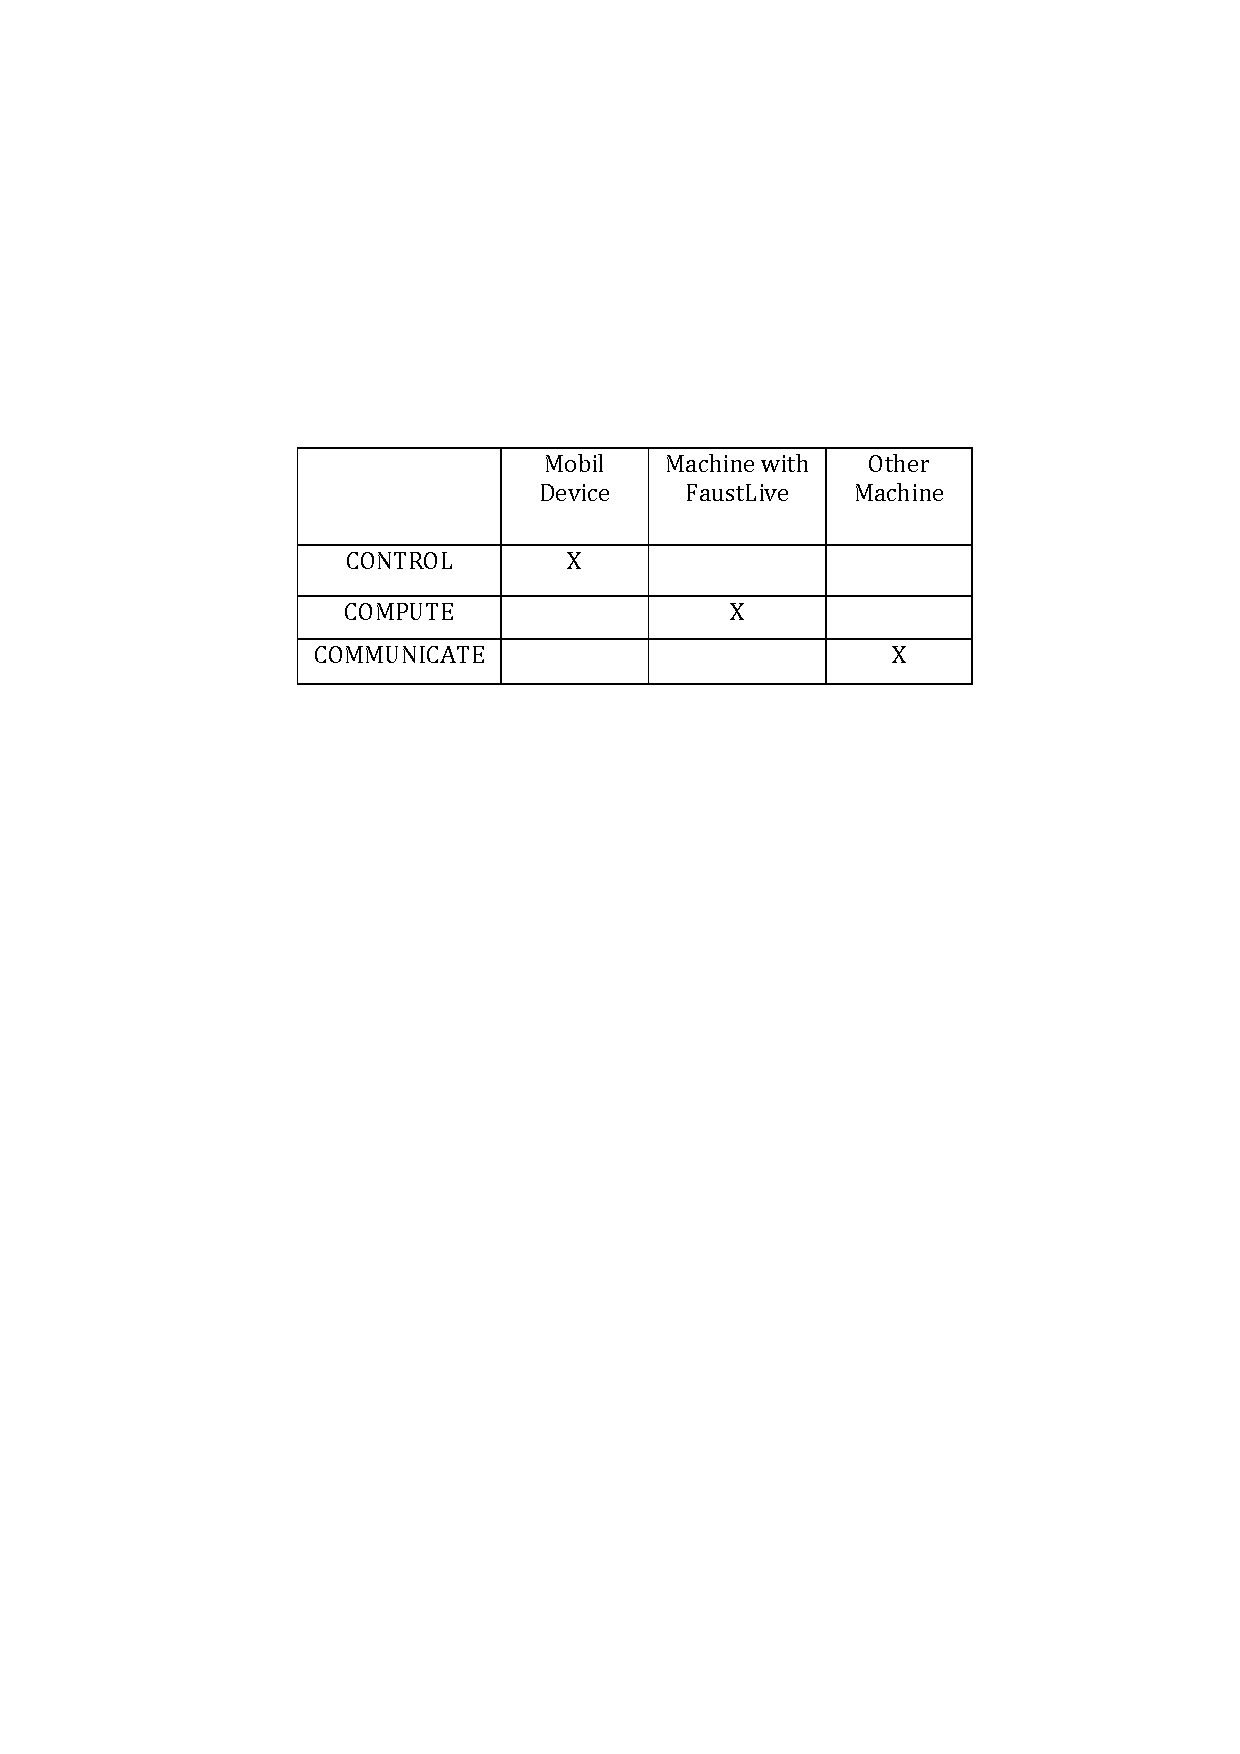
\includegraphics[width=0.7\columnwidth]{images/8CCC}
\caption{Control-Compute-Communicate Division with remote control and remote audio rendering}
\label{fig:8CCC}
\end{center}
\end{figure}
\begin{figure}[!h]
\begin{center}
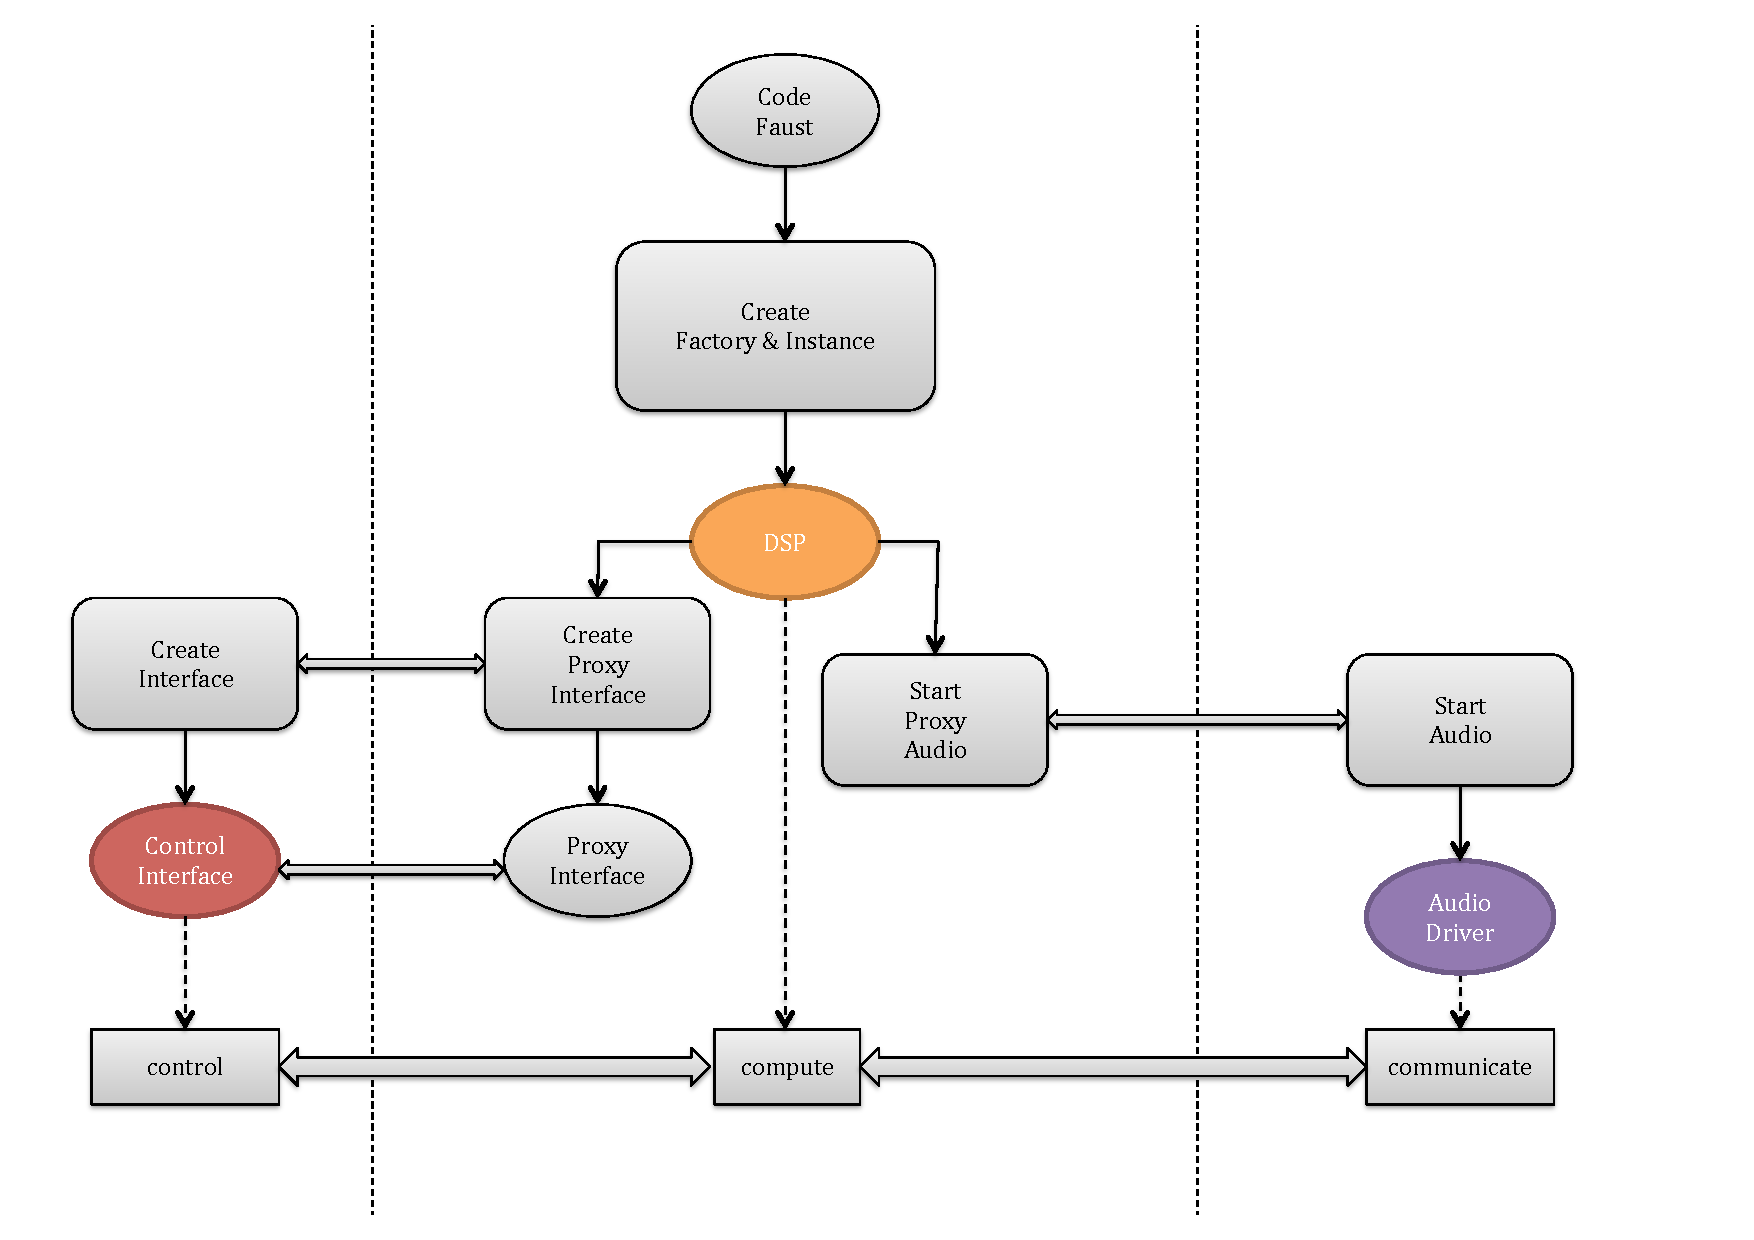
\includegraphics[width=\columnwidth]{images/CCC8}
\caption{Creation of the Interface/DSP/Driver for a remote control and rendering use case}
\label{fig:CCC8}
\end{center}
\end{figure}

%%%%%%%%%%%%%%REMOTE PROCESSING%%%%%%%%%%%%%%%%%
\newpage
\subsection {Remote processing} \label{remoteprocessing}

1 use case is implemented in FaustLive:
\begin{itemize}
\item FaustLive sends code to create a remote factory then uses its proxy DSP to create the control interface and communicate with the audio driver.
\end{itemize}
You can access this use case through the scrolling menu containing the available servers below the window. \\

The 2nd use case is conceivable but not implemented:
\begin{itemize}
\item FaustLive discovers remote servers and its available factories. Then it can request a remote instance then uses the proxy DSP to create the interface and communicate with the audio driver.
\end{itemize}

\begin{figure}[!h]
\begin{center}
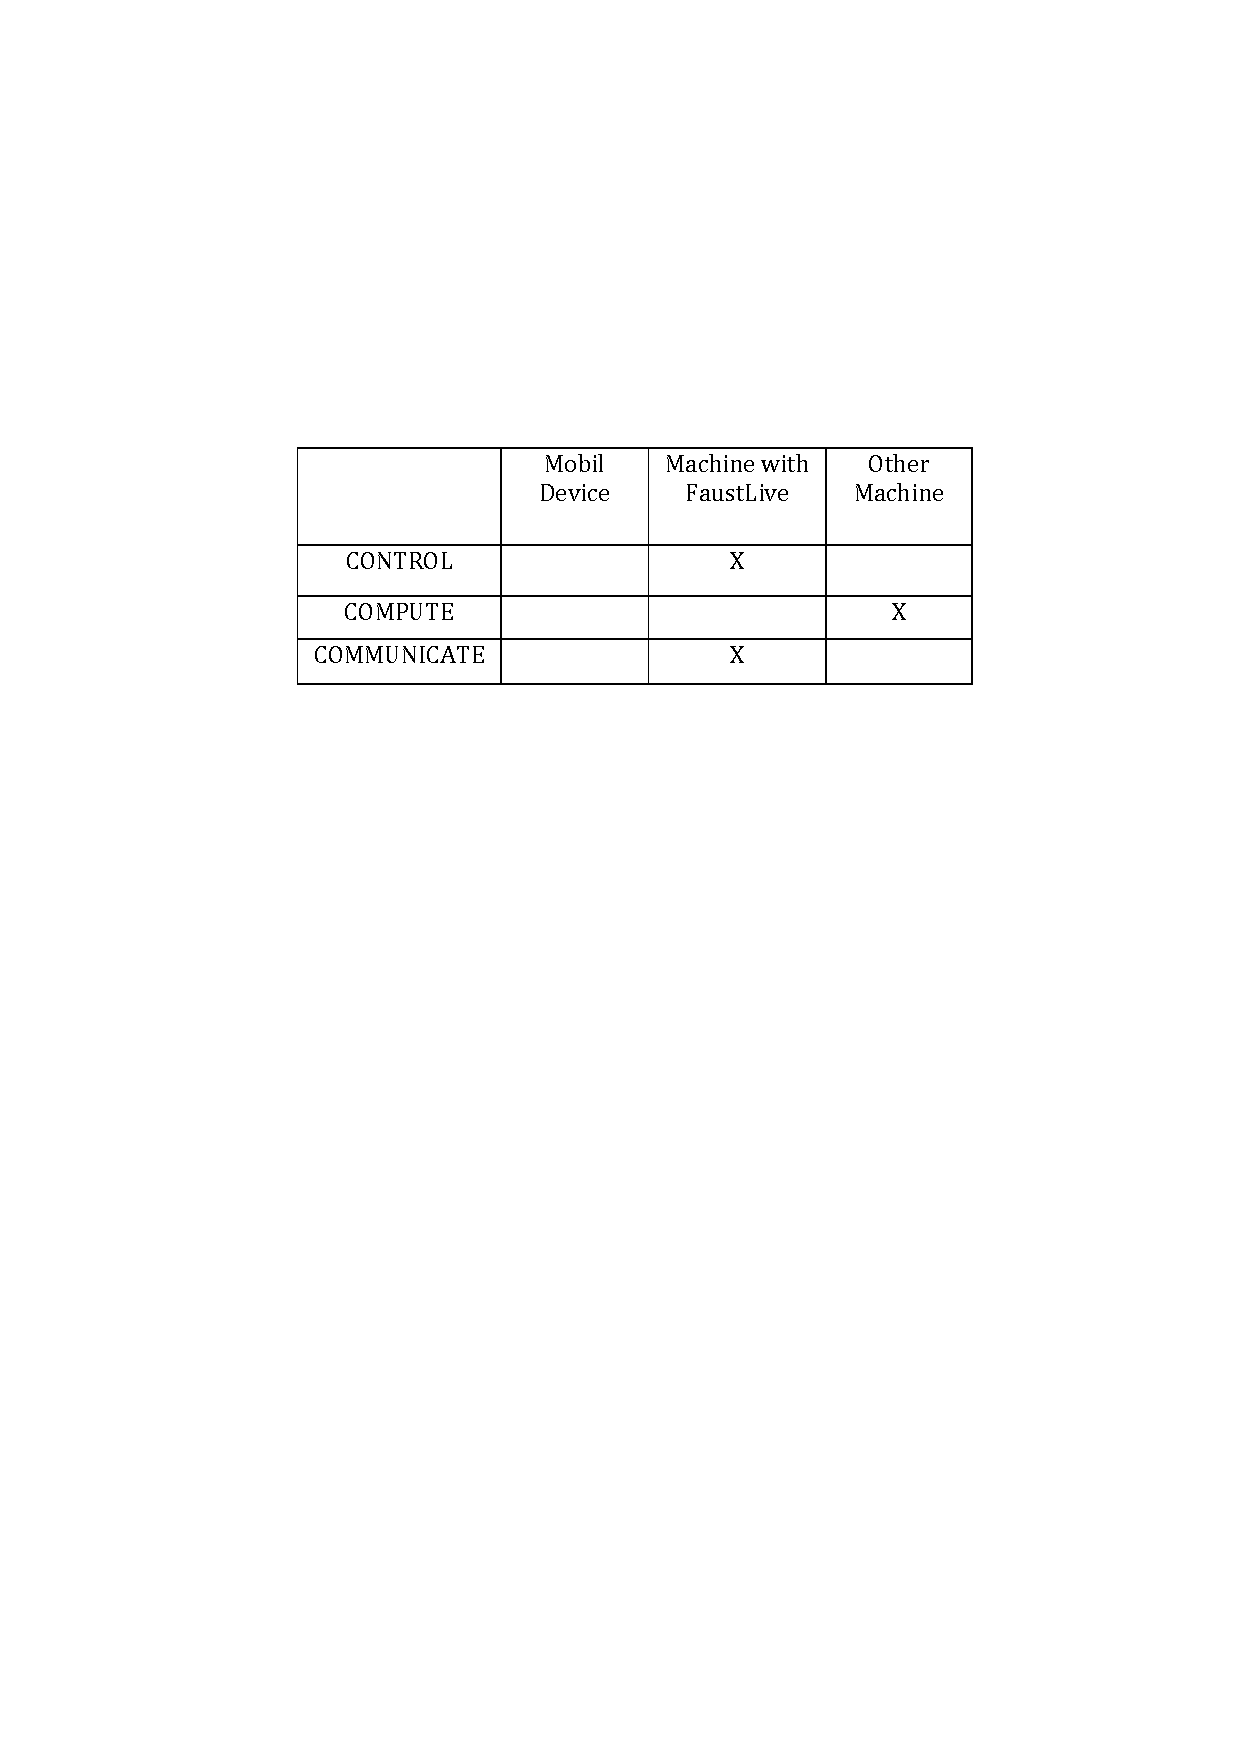
\includegraphics[width=0.7\columnwidth]{images/4CCC}
\caption{Control-Compute-Communicate Division with remote processing}
\label{fig:4CCC}
\end{center}
\end{figure}
\begin{figure}[!h]
\begin{center}

\begin{minipage}[c]{.45\linewidth}
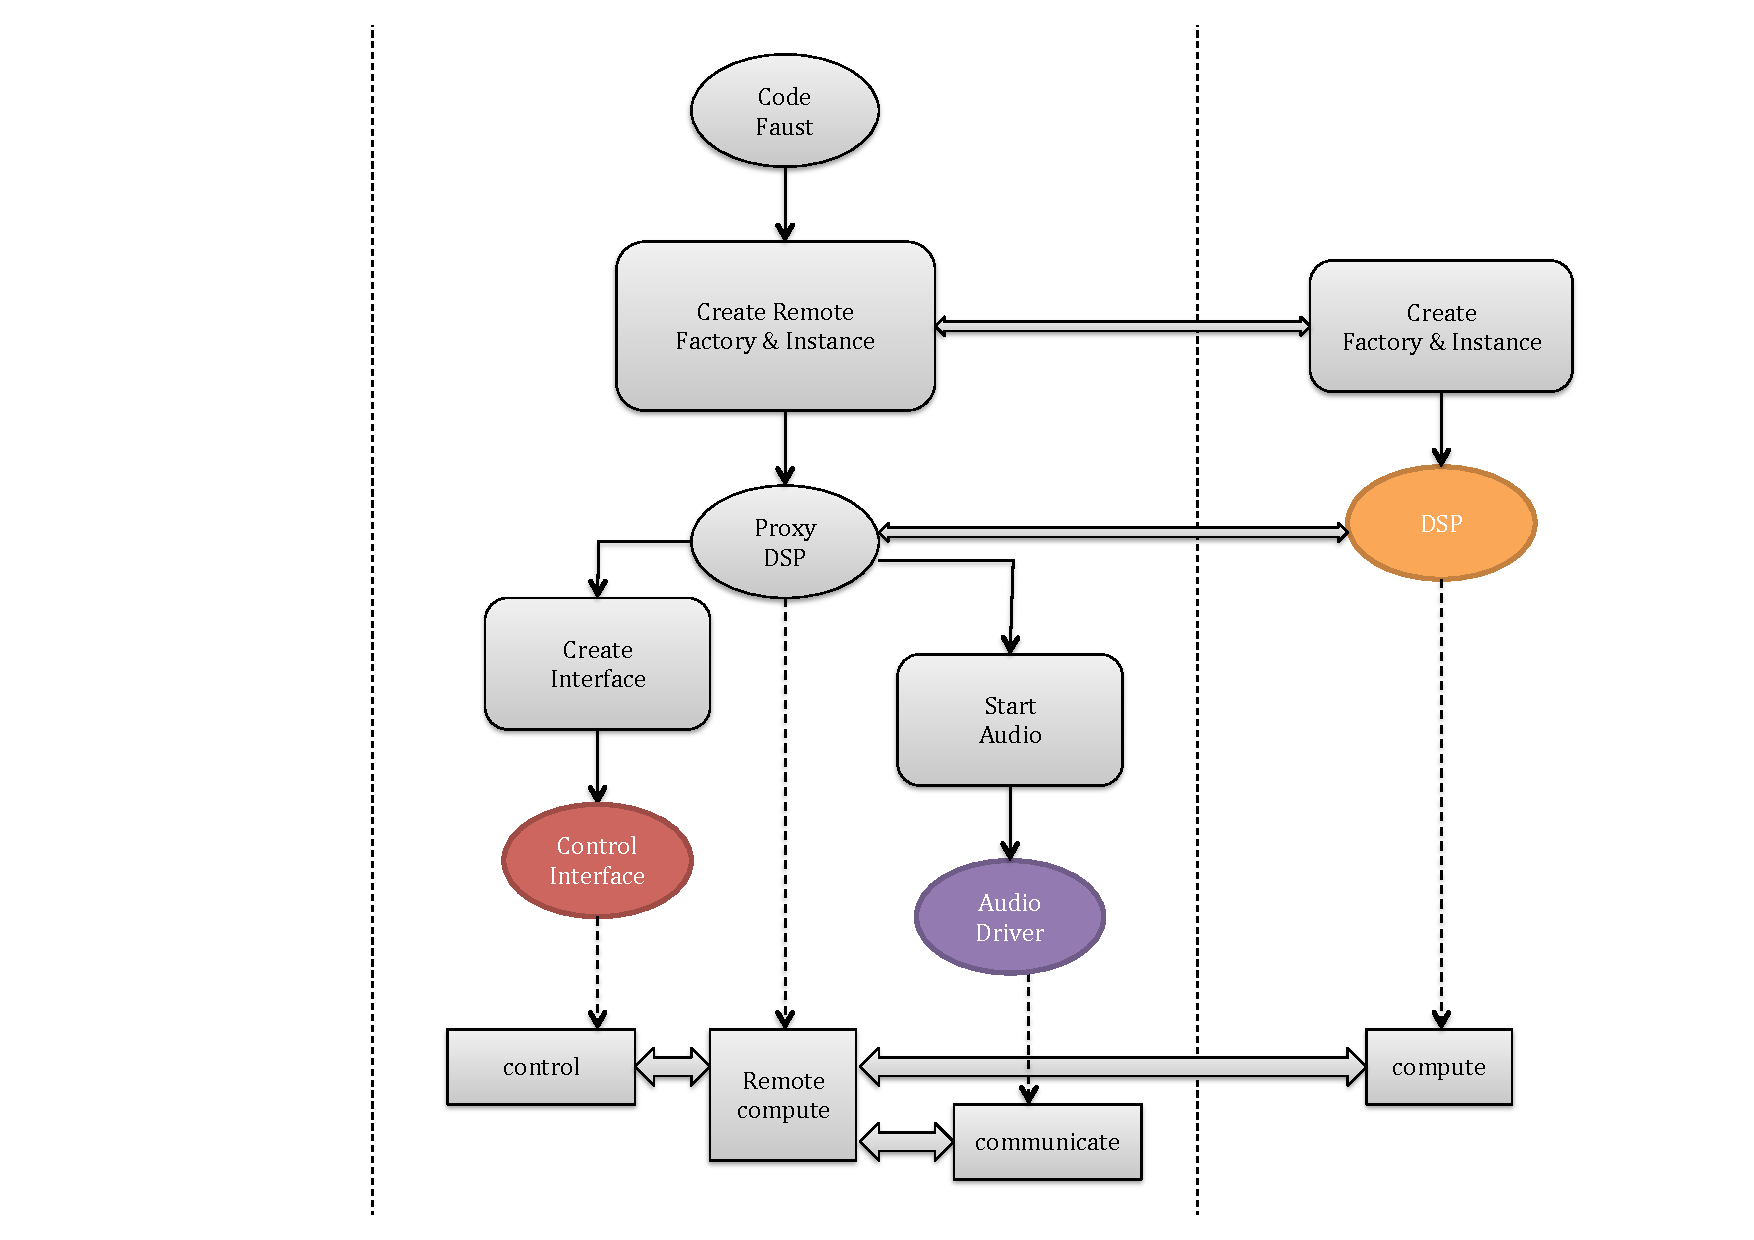
\includegraphics[width=\columnwidth]{images/CCC41}
\end{minipage}
\begin{minipage}[r]{.45\linewidth}
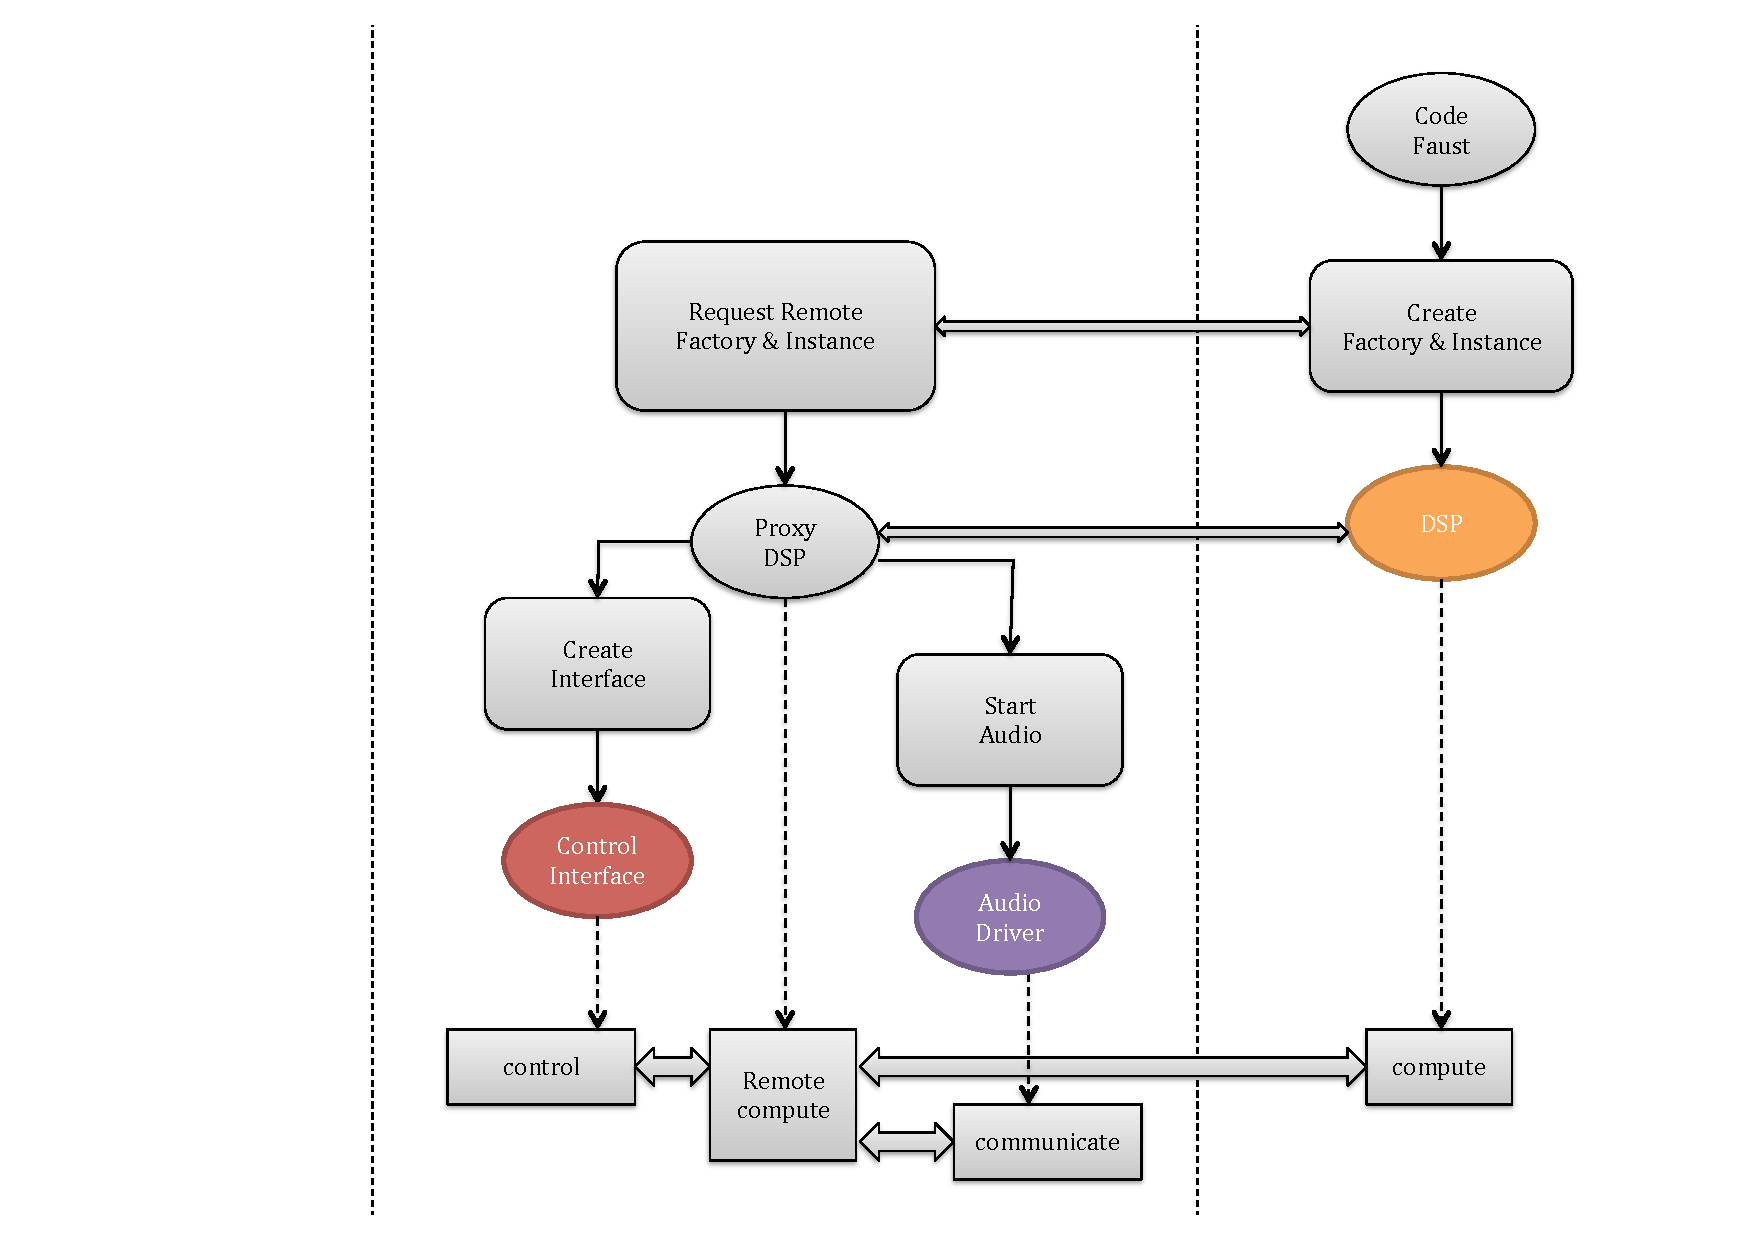
\includegraphics[width=\columnwidth]{images/CCC42}
\end{minipage}
\caption{Creation of the Interface/DSP/Driver for a remote processing use case}
\label{fig:CCC4}
\end{center}
\end{figure}

%%%%%%%%%%%%%%REMOTE PROCESSING AND CONTROL%%%%%%%%%%%%%%%%%
\newpage
\subsection{ Remote processing and remote control}

Combining use case {\ref{remotecontrol}} and use case {\ref{remoteprocessing}}.

1 use case is implemented in FaustLive:
\begin{itemize}
\item use the OSC or HTTP control combined with the remote processing, code sended by FaustLive.
\end{itemize}

The imaginary use cases are all combination of the imaginary use cases of {\ref{remotecontrol}} and {\ref{remoteprocessing}}.

\begin{figure}[!h]
\begin{center}
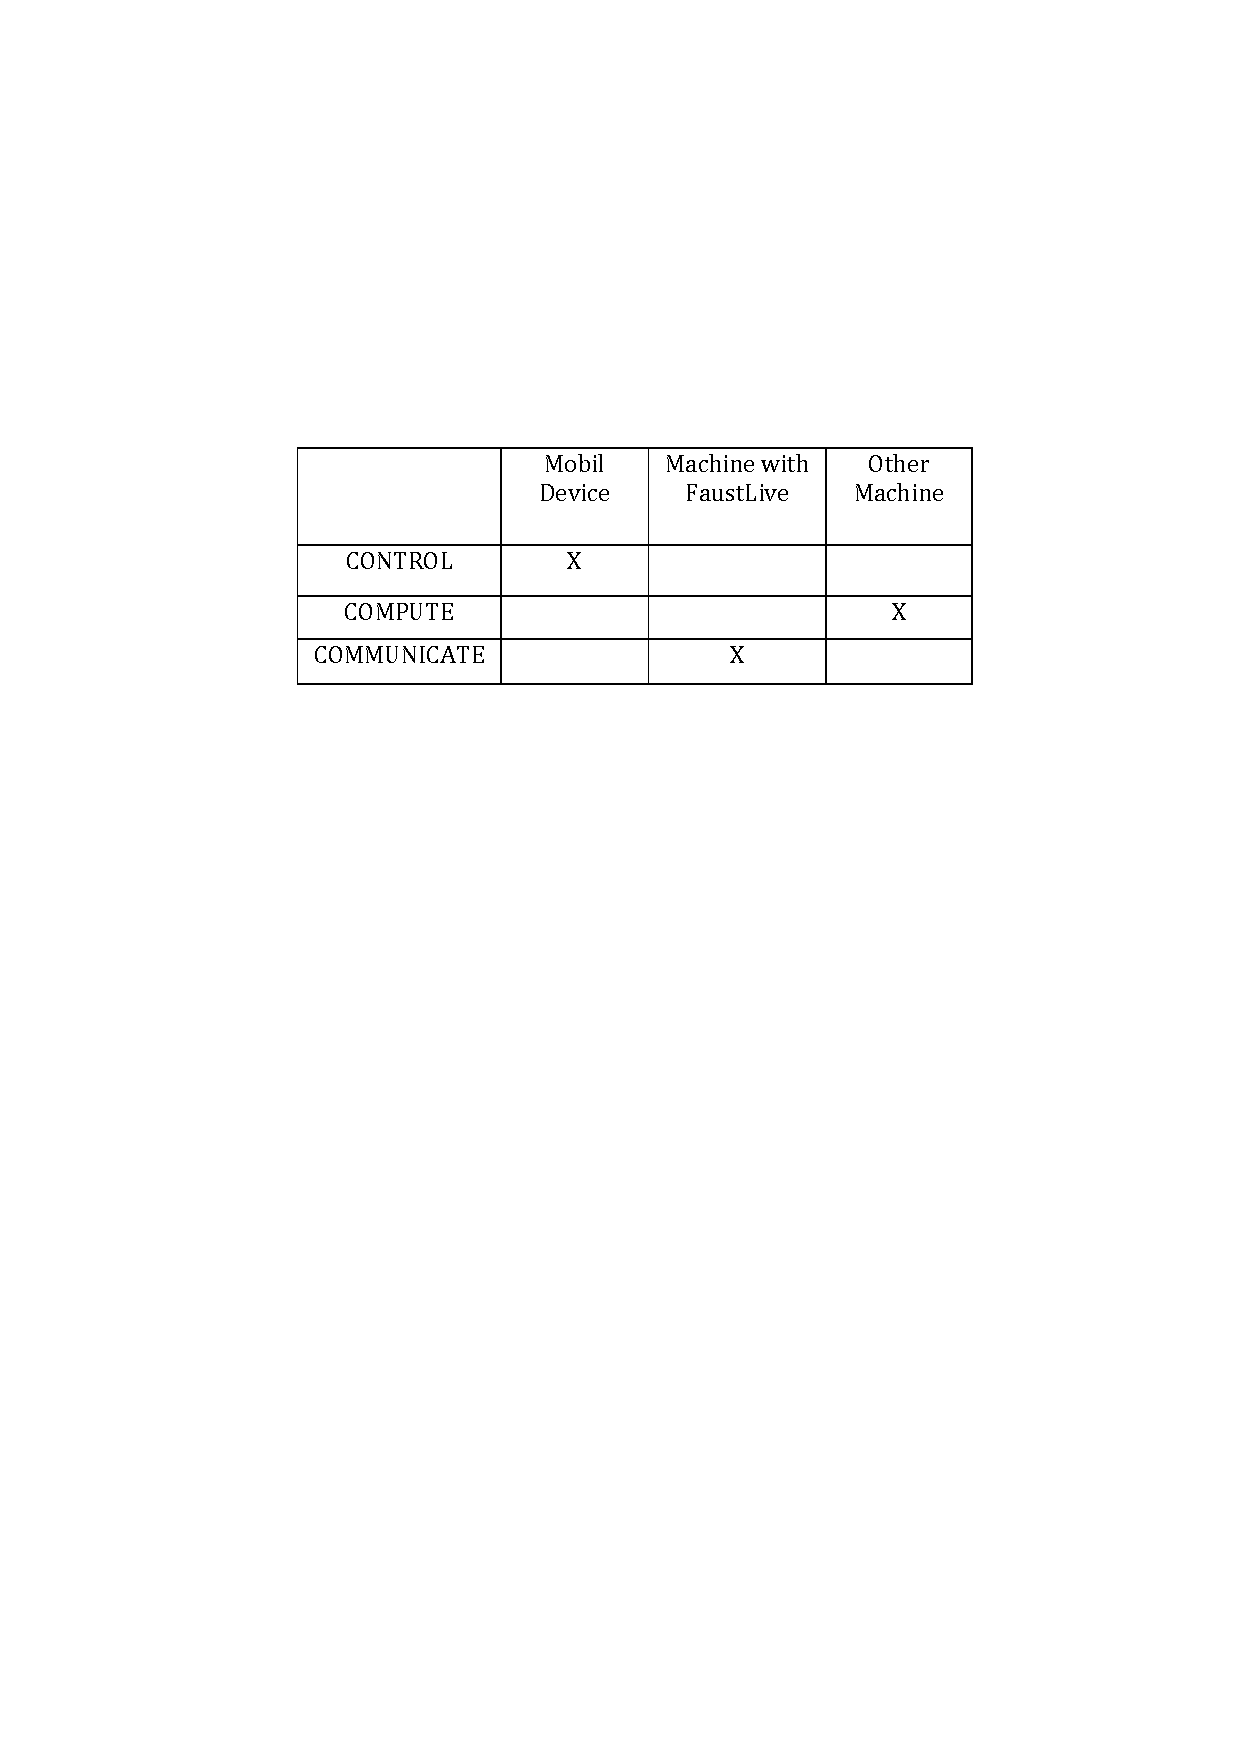
\includegraphics[width=0.7\columnwidth]{images/5CCC}
\caption{Control-Compute-Communicate Division with remote processing and control}
\label{fig:5CCC}
\end{center}
\end{figure}

\begin{figure}[!h]
\begin{center}
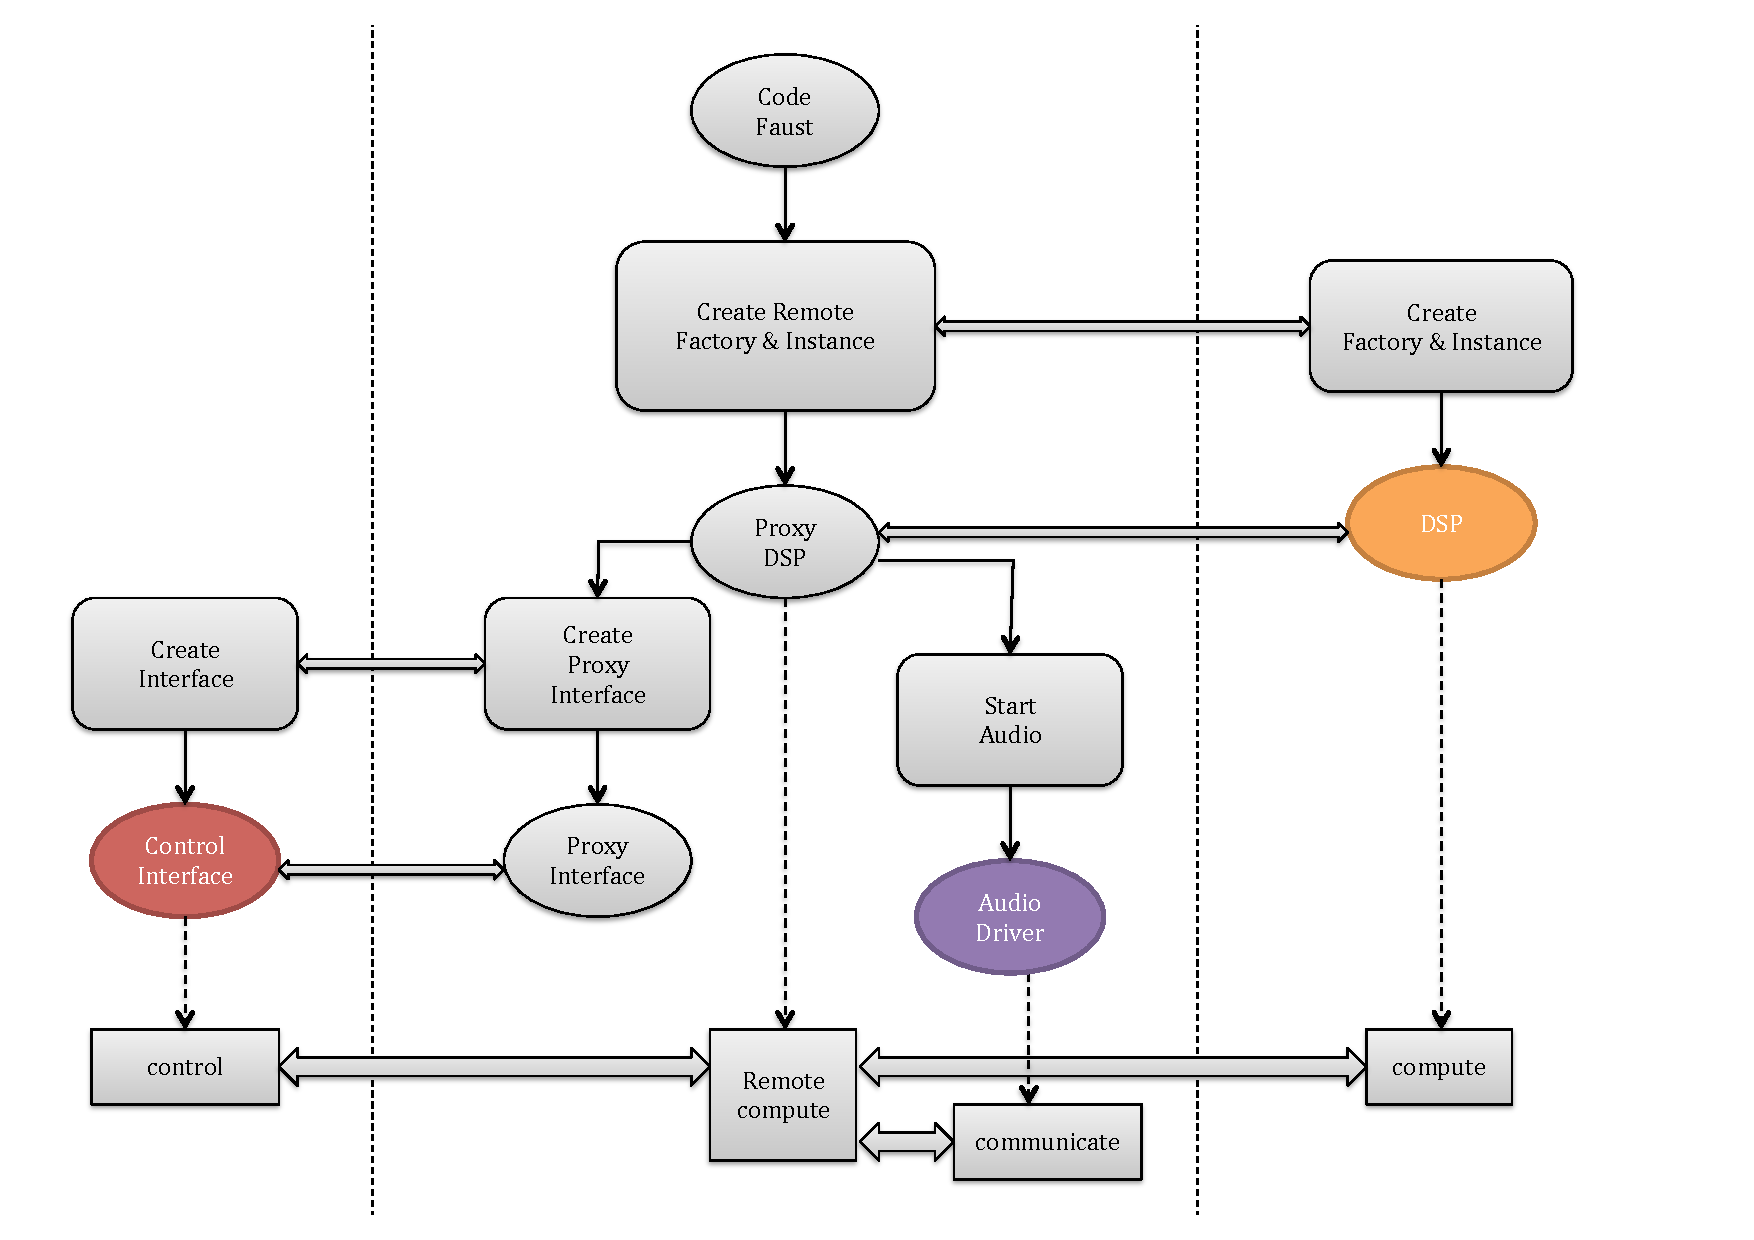
\includegraphics[width=\columnwidth]{images/CCC5}
\caption{Creation of the Interface/DSP/Driver for a remote processing and control}
\label{fig:CCC8}
\end{center}
\end{figure}


%%%%%%%%%%%%%%REMOTE PROCESSING AND RENDERING%%%%%%%%%%%%%%%%%
\newpage
\subsection{ Remote processing and remote rendering}

The remote processing use cases are described on {\ref {remoteprocessing}}. \\

1 use case is implemented in FaustLive:
\begin{itemize}
\item NetJack is used to communicate between machines and render remotly. The communication between "Control" and "Communicate" runs through FaustLive. (combine \ref{remoterendering} and \ref{remoteprocessing})
\end{itemize}

The 2nd use case is conceivable but not implemented:
\begin{itemize}
\item The local driver (on the "Other Machine") is used to render. The communication between "Control" and "Communicate" does not run through FaustLive.
\end{itemize}

\begin{figure}[!h]
\begin{center}
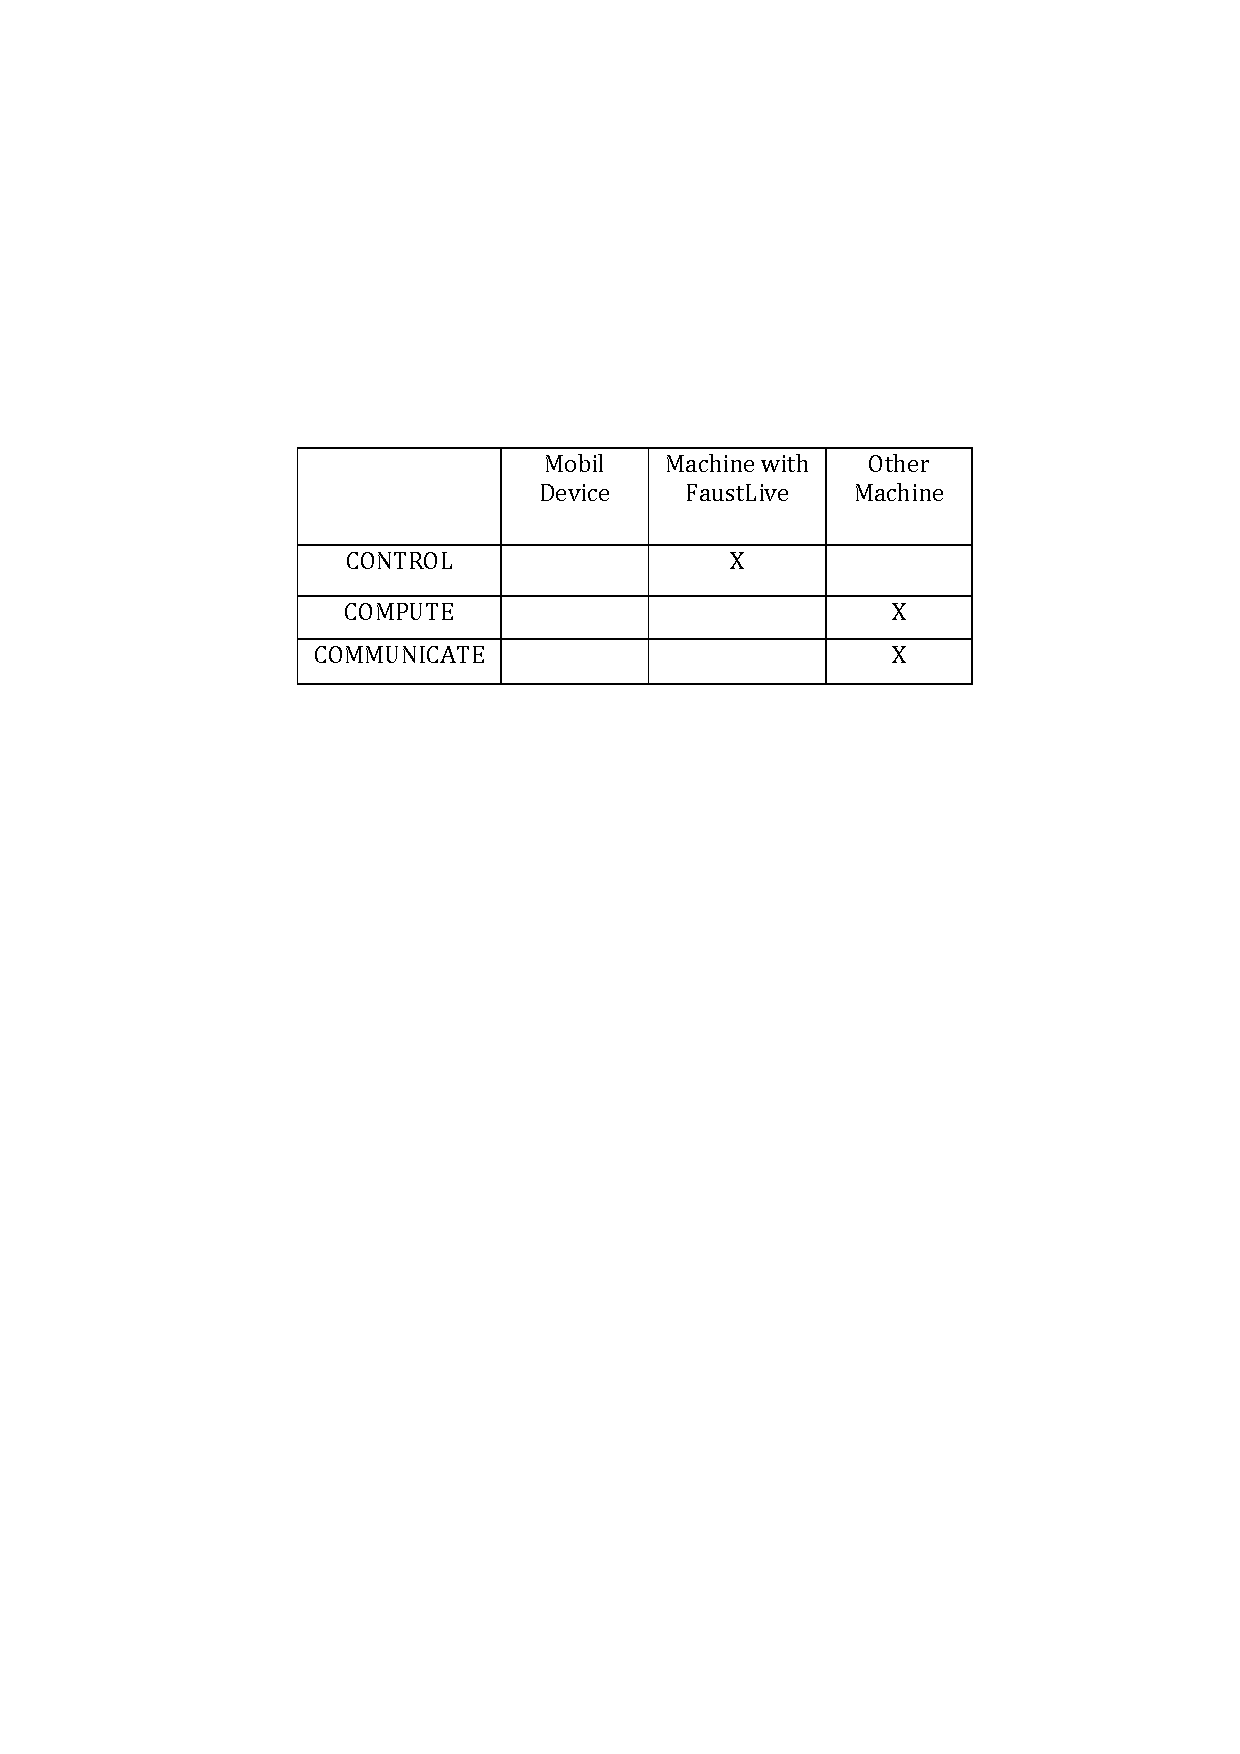
\includegraphics[width=0.7\columnwidth]{images/7CCC}
\caption{Control-Compute-Communicate Division with remote processing and remote audio rendering}
\label{fig:7CCC}
\end{center}
\end{figure}

\begin{figure}[!h]
\begin{center}
\begin{minipage}[c]{.45\linewidth}
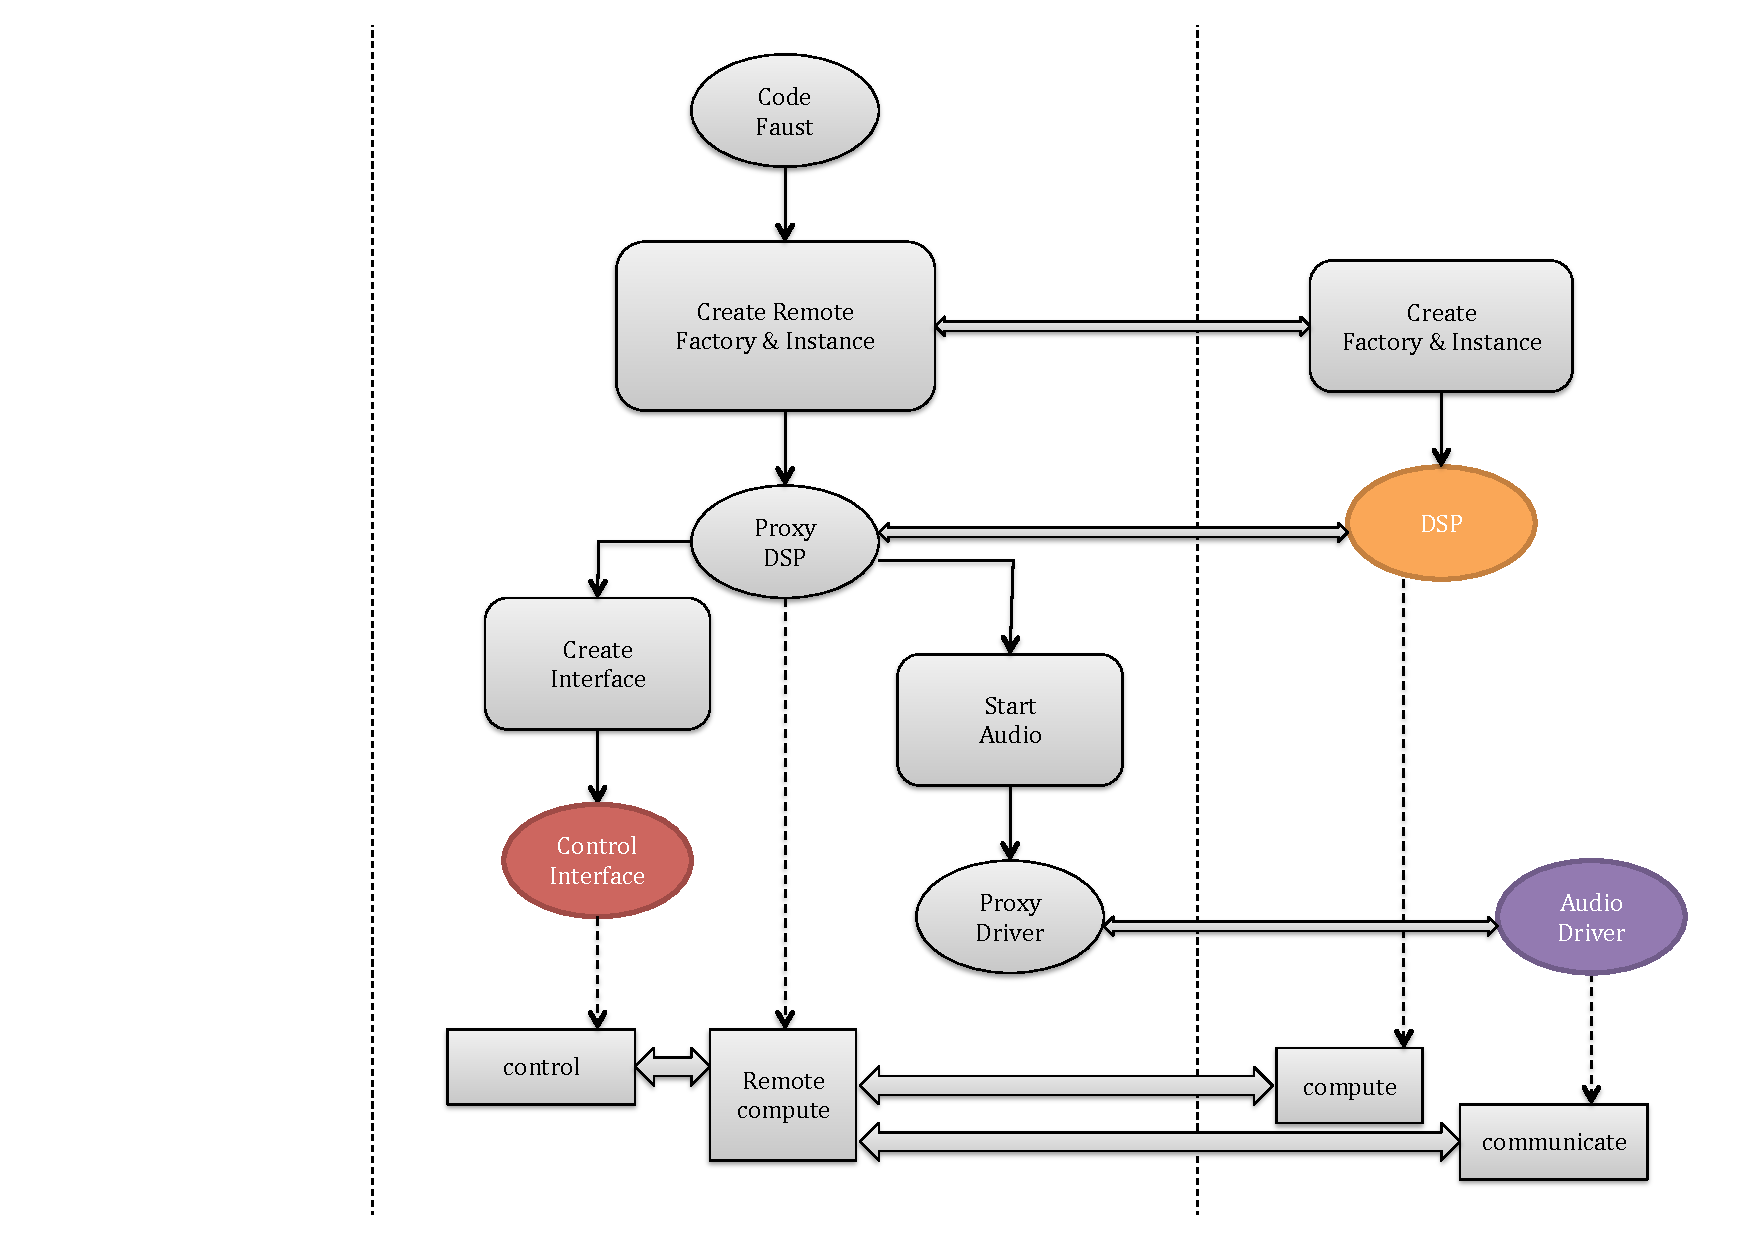
\includegraphics[width=\columnwidth]{images/CCC71}
\end{minipage}
\begin{minipage}[r]{.45\linewidth}
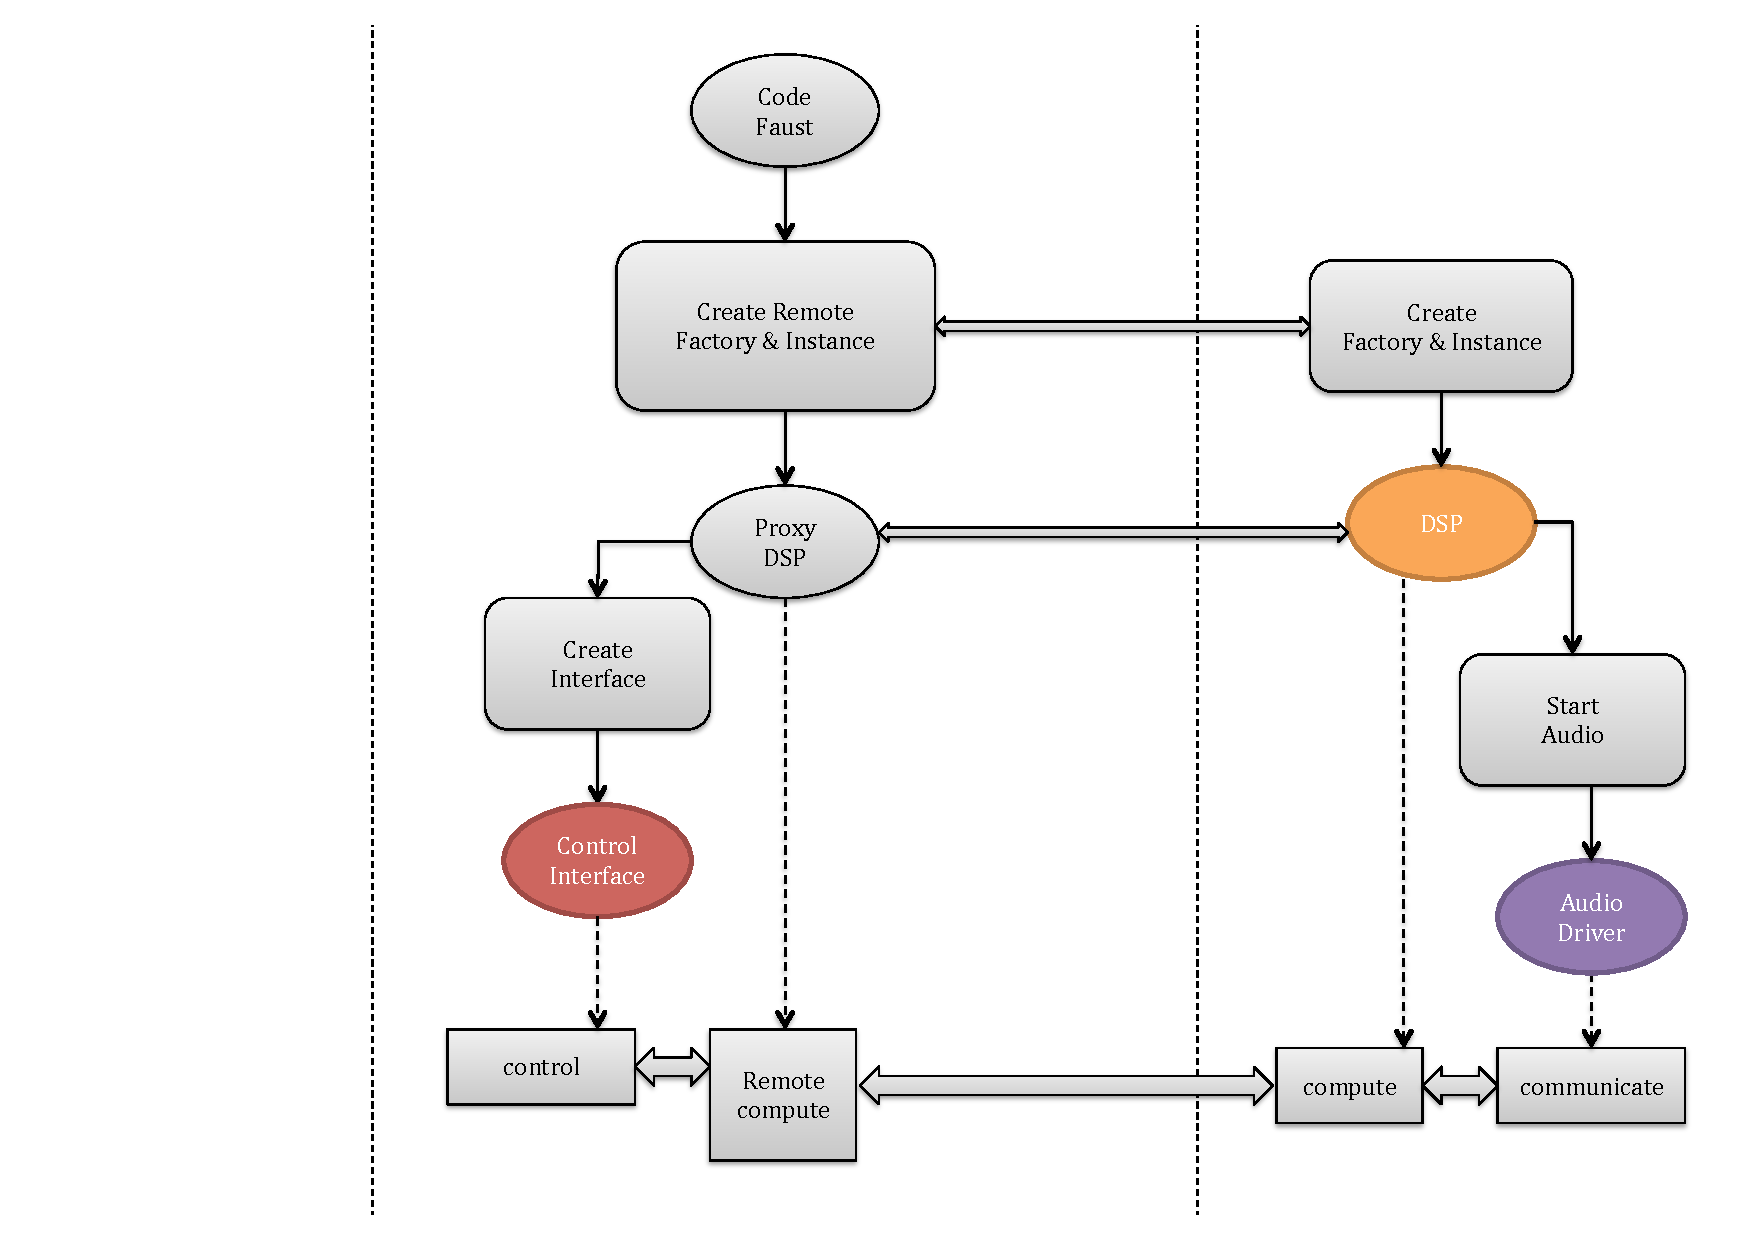
\includegraphics[width=\columnwidth]{images/CCC72}
\end{minipage}
\caption{Creation of the Interface/DSP/Driver for a remote processing and rendering use case}
\label{fig:CCC4}
\end{center}
\end{figure}

%%%%%%%%%%%%%%REMOTE CONTROL AND RENDERING ON MOBILE DEVICE%%%%%%%%%%%%%%%%%
\newpage
\subsection{ Remote processing from remote device}

This is the opposite of use case {\ref {remoteprocessing}} from FaustLive point of view. \\
This is the same use case {\ref {remoteprocessing}} from the remote device point of view. \\

The mobile device discovers remote factories on FaustLive and requests a remote instance then uses its proxy DSP to create the control interface and communicate with the audio driver. \\
This use case is "more or less" available in FaustLive. The trick is to switch to a local remote processing server. The factory is then public on the server and accessible for remote devices. The remote instance is totally independent from the local instance. It just uses the server running in FaustLive. It would be nice to rethink this, in order to share the same system of Factory/Instance creation (in FLSessionManager). \\

An idea would be to have the possibility to "publish" the factory without quitting the local processing of the current running DSP. \\
Another one is the possibility to create the factory from the mobile device is represented on Figure 14, left part.

\begin{figure}[!h]
\begin{center}
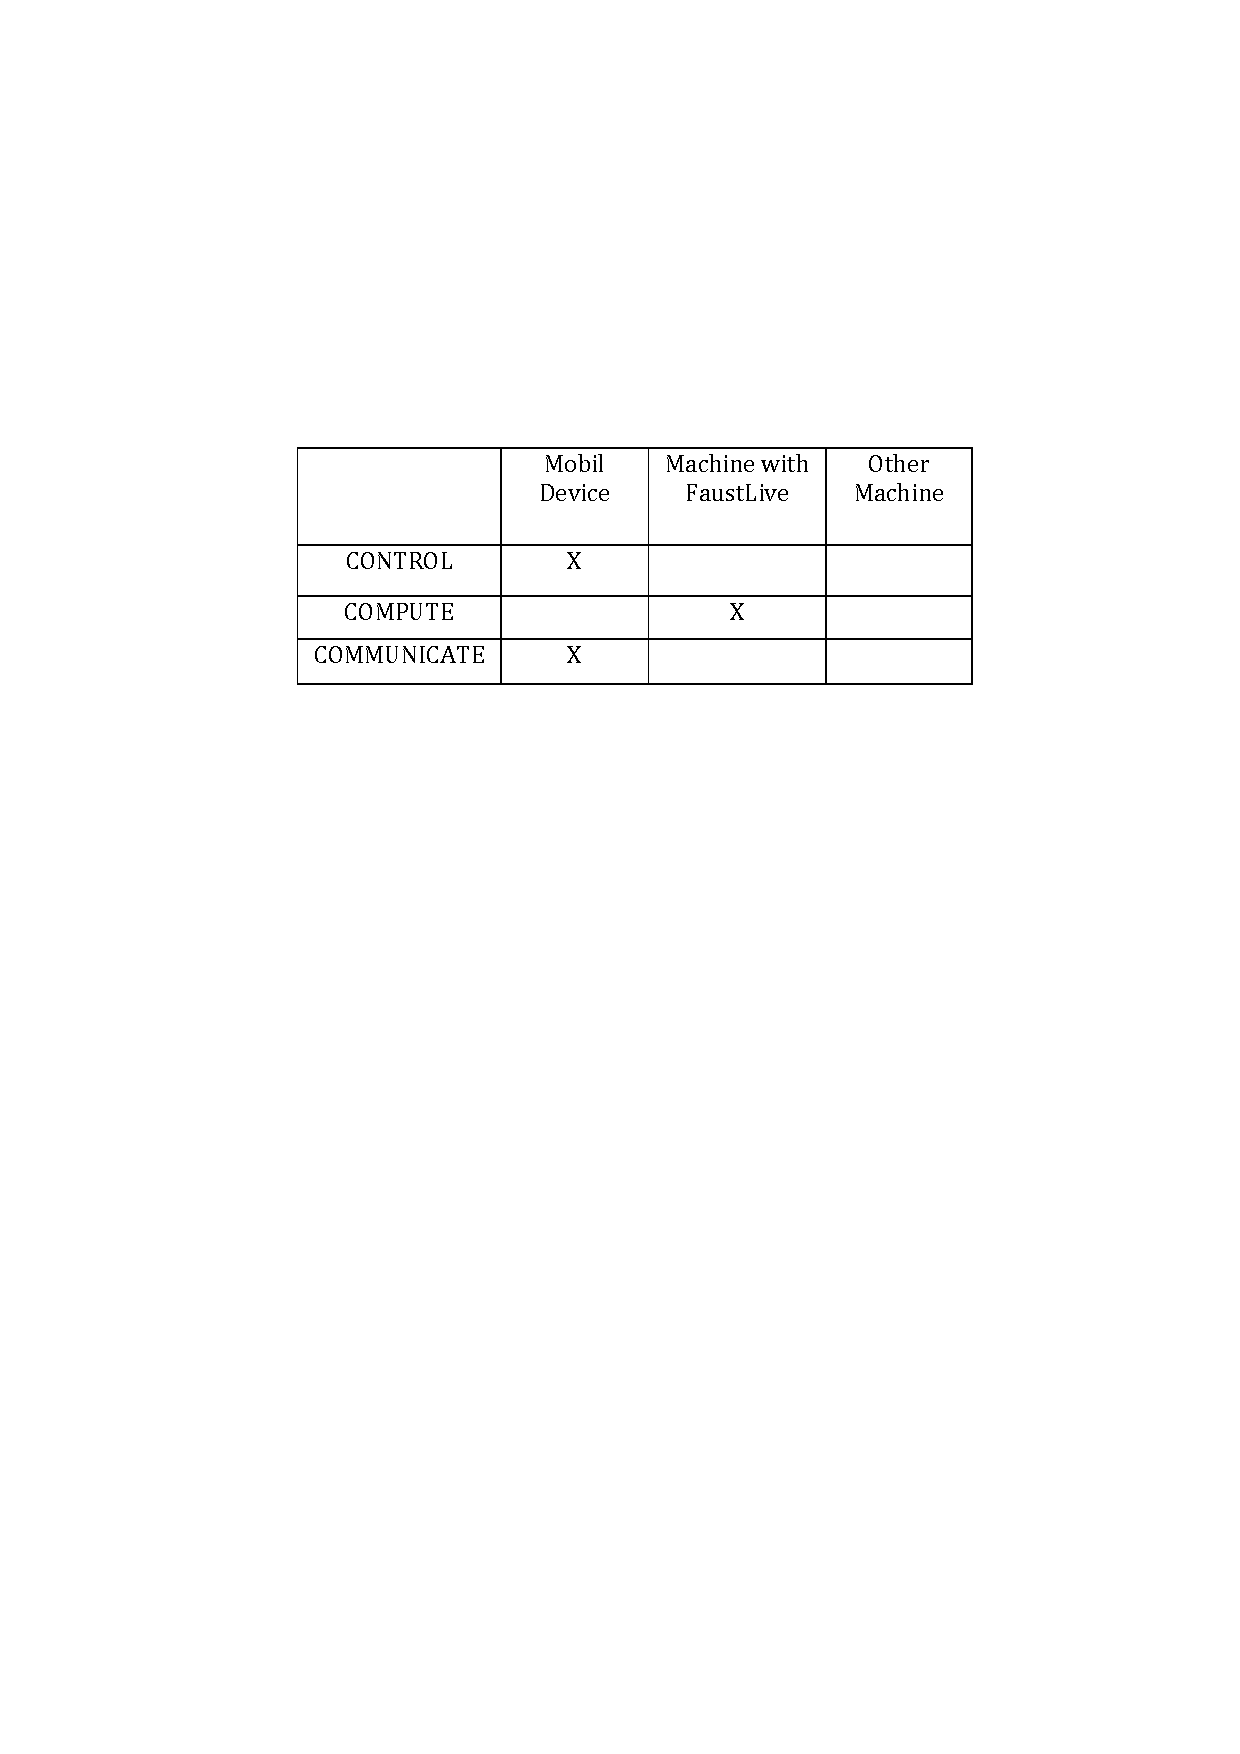
\includegraphics[width=0.7\columnwidth]{images/6CCC}
\caption{Control-Compute-Communicate Division with mobile device use case}
\label{fig:6CCC}
\end{center}
\end{figure}

\begin{figure}[!h]
\begin{center}
\begin{minipage}[c]{.45\linewidth}
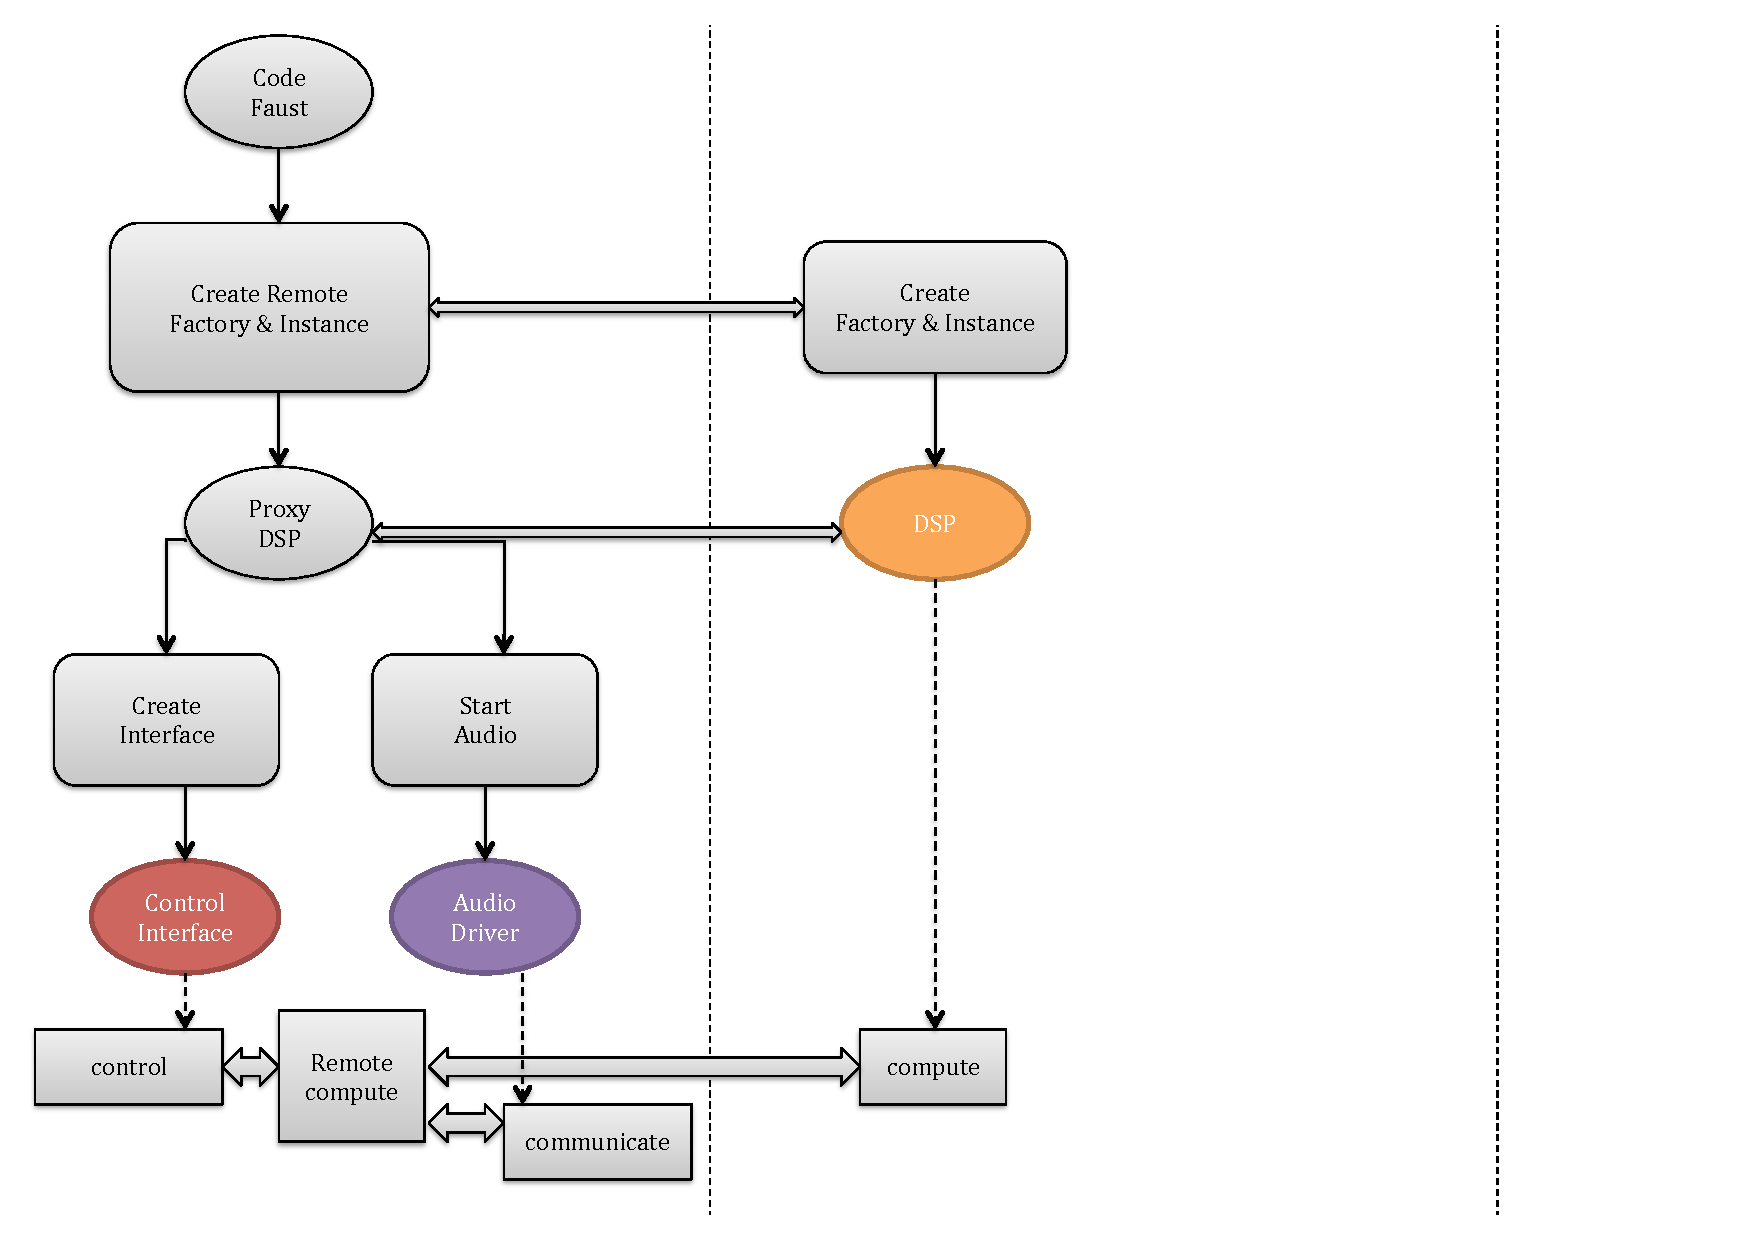
\includegraphics[width=\columnwidth]{images/CCC61}
\end{minipage}
\begin{minipage}[r]{.45\linewidth}
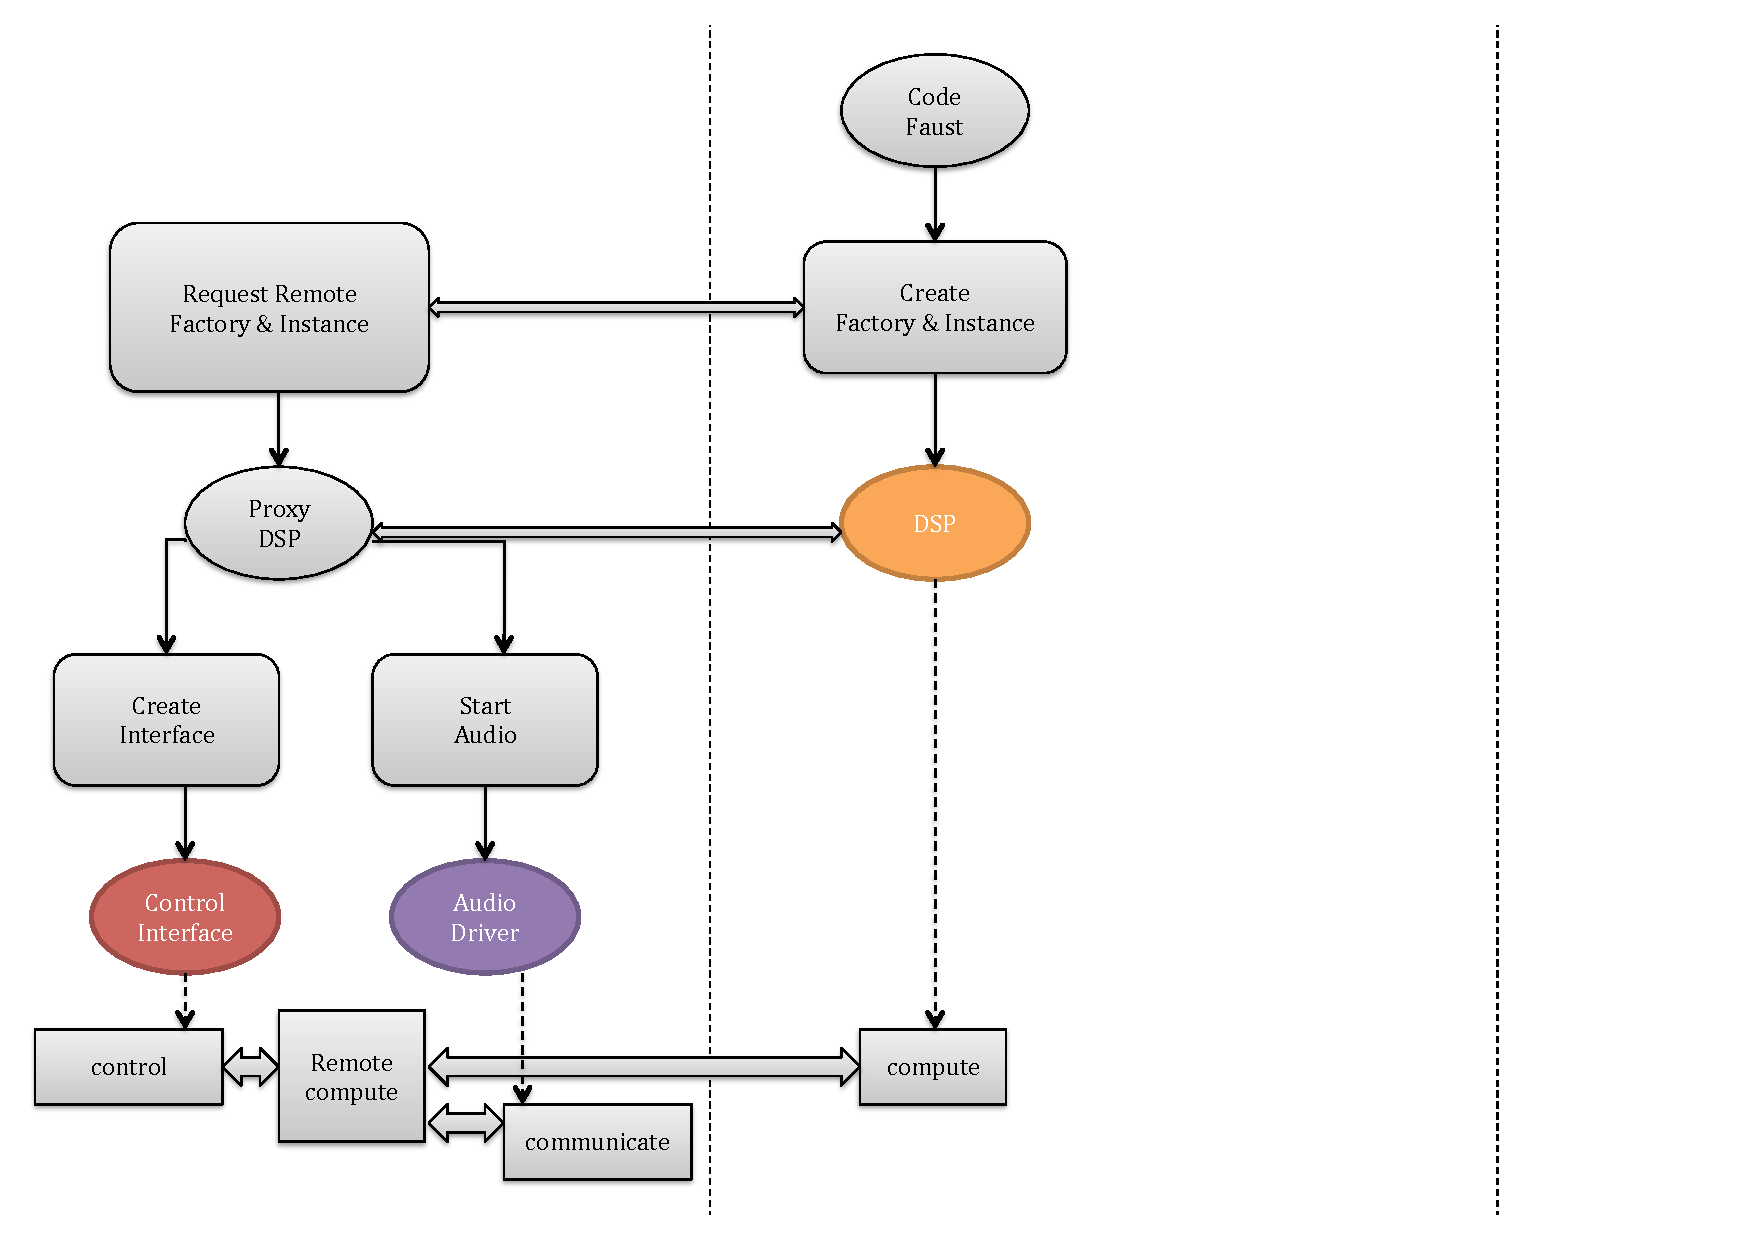
\includegraphics[width=\columnwidth]{images/CCC62}
\end{minipage}
\caption{Creation of the Interface/DSP/Driver for a remote control and rendering on a mobile device}
\label{fig:CCC4}
\end{center}
\end{figure}

\subsection{Synchronized remote processing from remote device}\label{synchronizedremote}

Another important aspect would be to have the possibility to synchronize the remote DSP with the FaustLive DSP. \\

In this use case, the remote device is synchronized with FaustLive interface. In case the source code changes, the remote interface is notified and recharged. 

\begin{figure}[!h]
\begin{center}
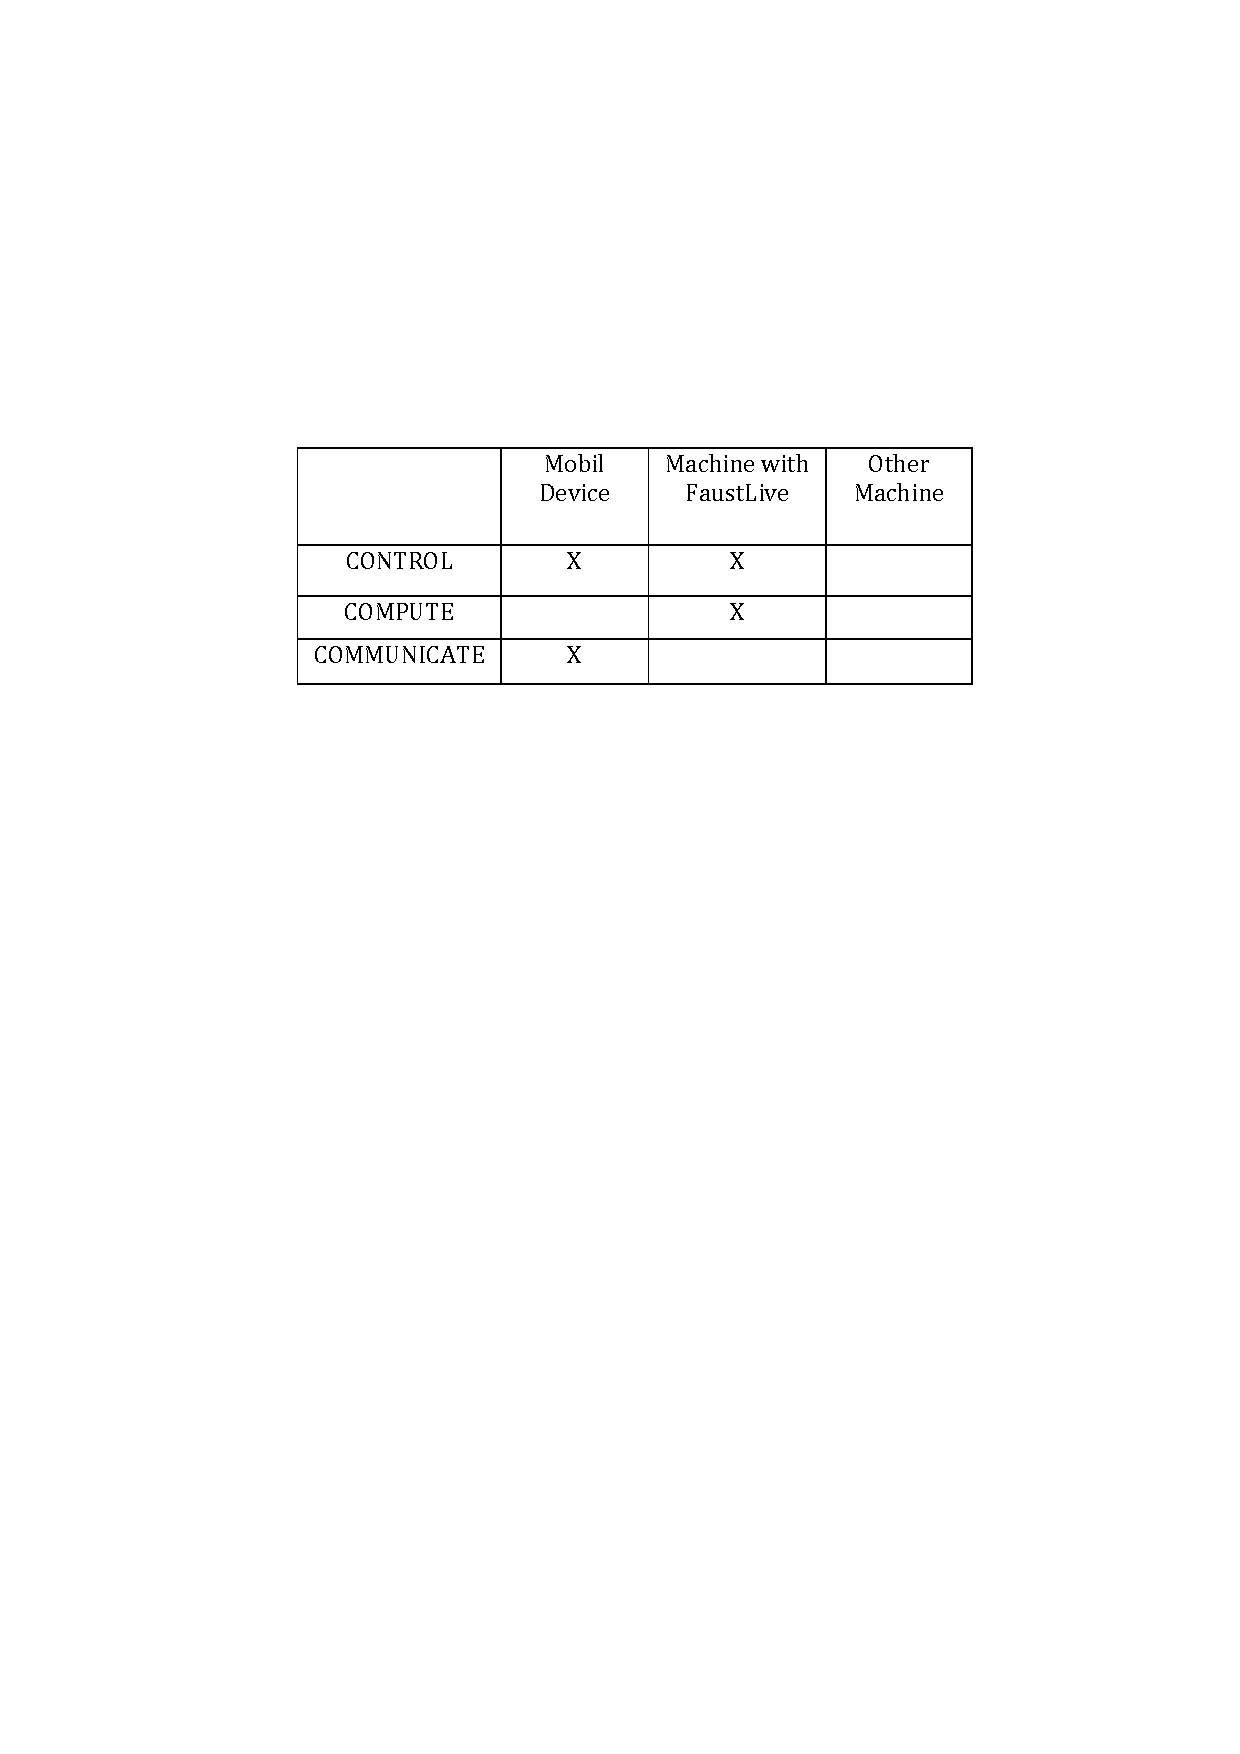
\includegraphics[width=0.7\columnwidth]{images/61CCC}
\caption{Control-Compute-Communicate Division with mobile device use case}
\label{fig:6CCC}
\end{center}
\end{figure}

\newpage
\subsection{ Double remote processing}\label{doubleprocessing}

This use case arises from use case \ref{synchronizedremote}. It imagines switching to a remote server machine while having a synchronized remote device. In this case, FaustLive is a server for the remote device and a client to the other machine.

\begin{figure}[!h]
\begin{center}
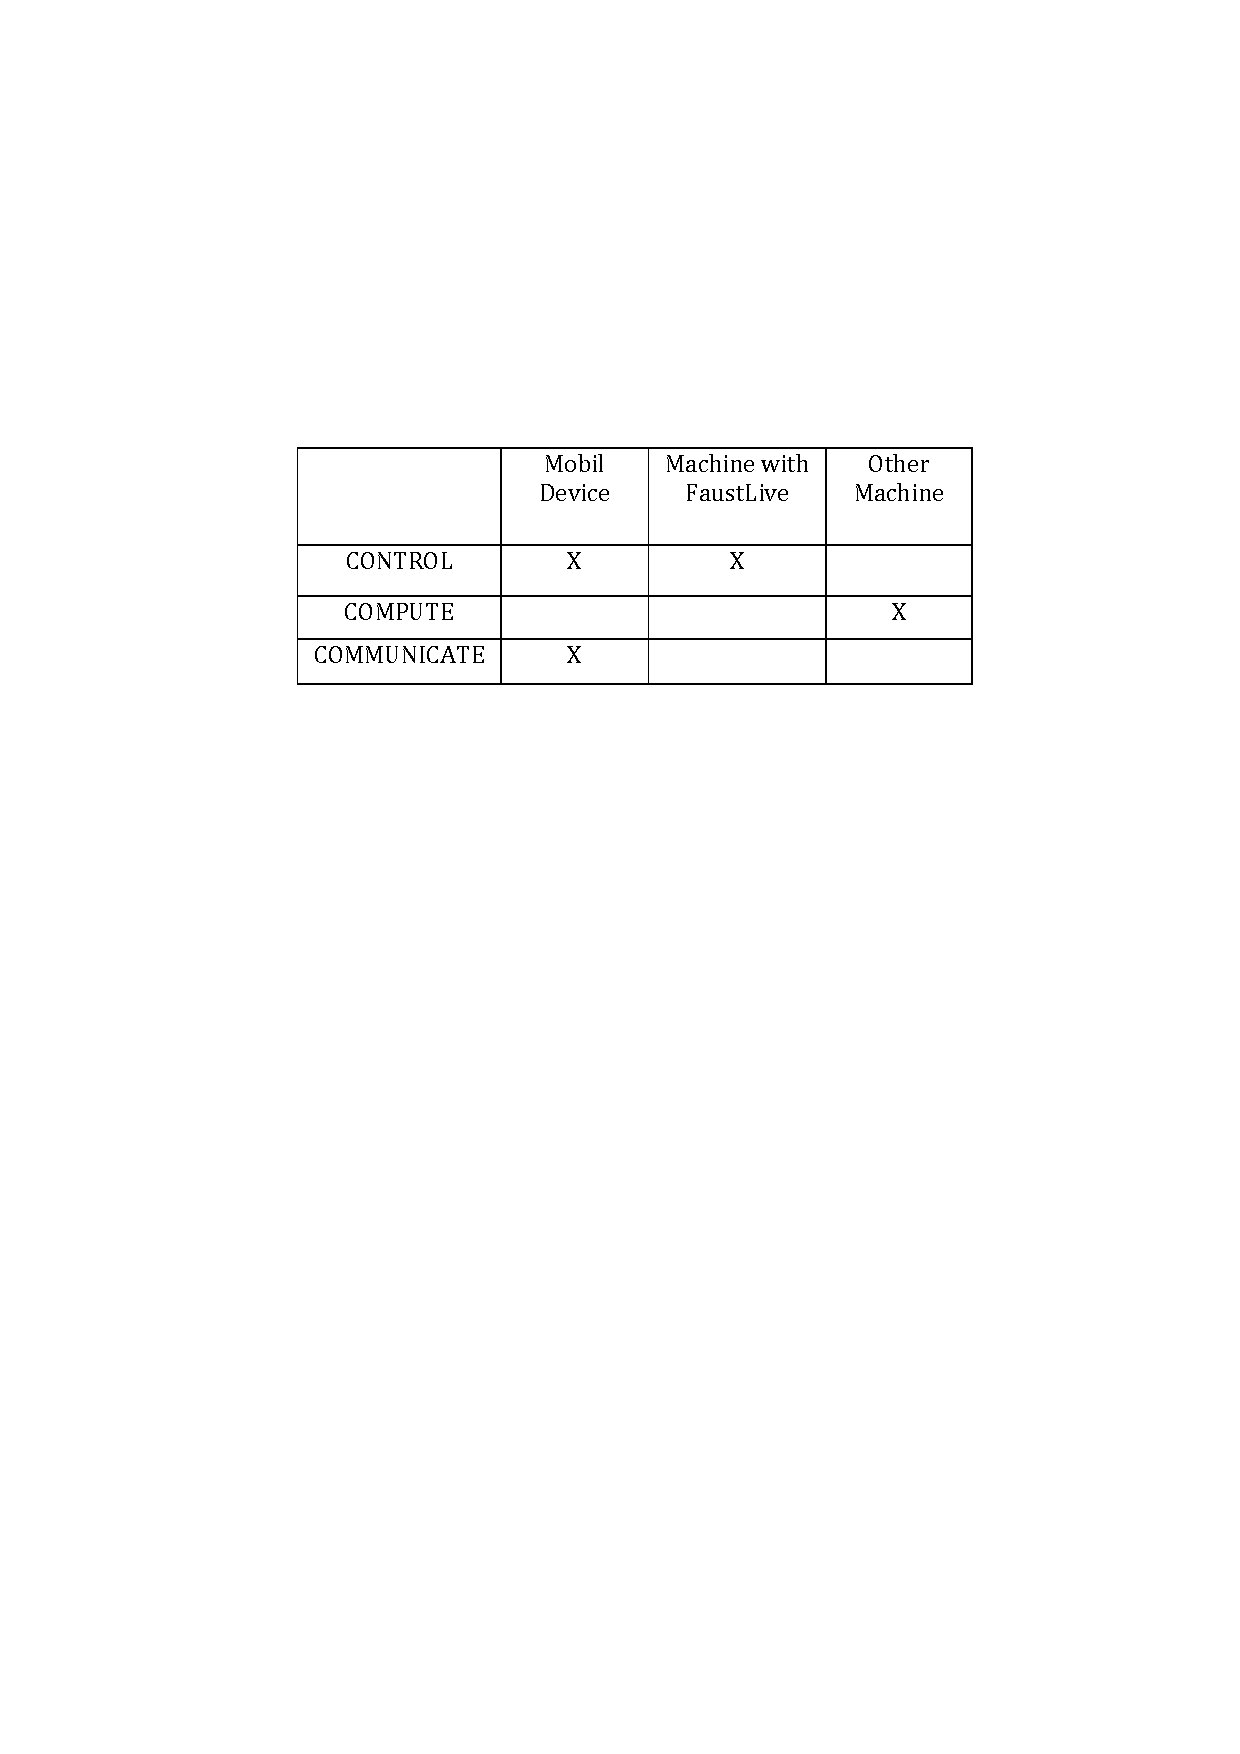
\includegraphics[width=0.7\columnwidth]{images/9CCC}
\caption{Control-Compute-Communicate Division with mobile device use case}
\label{fig:62CCC}
\end{center}
\end{figure}

\begin{figure}[!h]
\begin{center}
\begin{minipage}[c]{\linewidth}
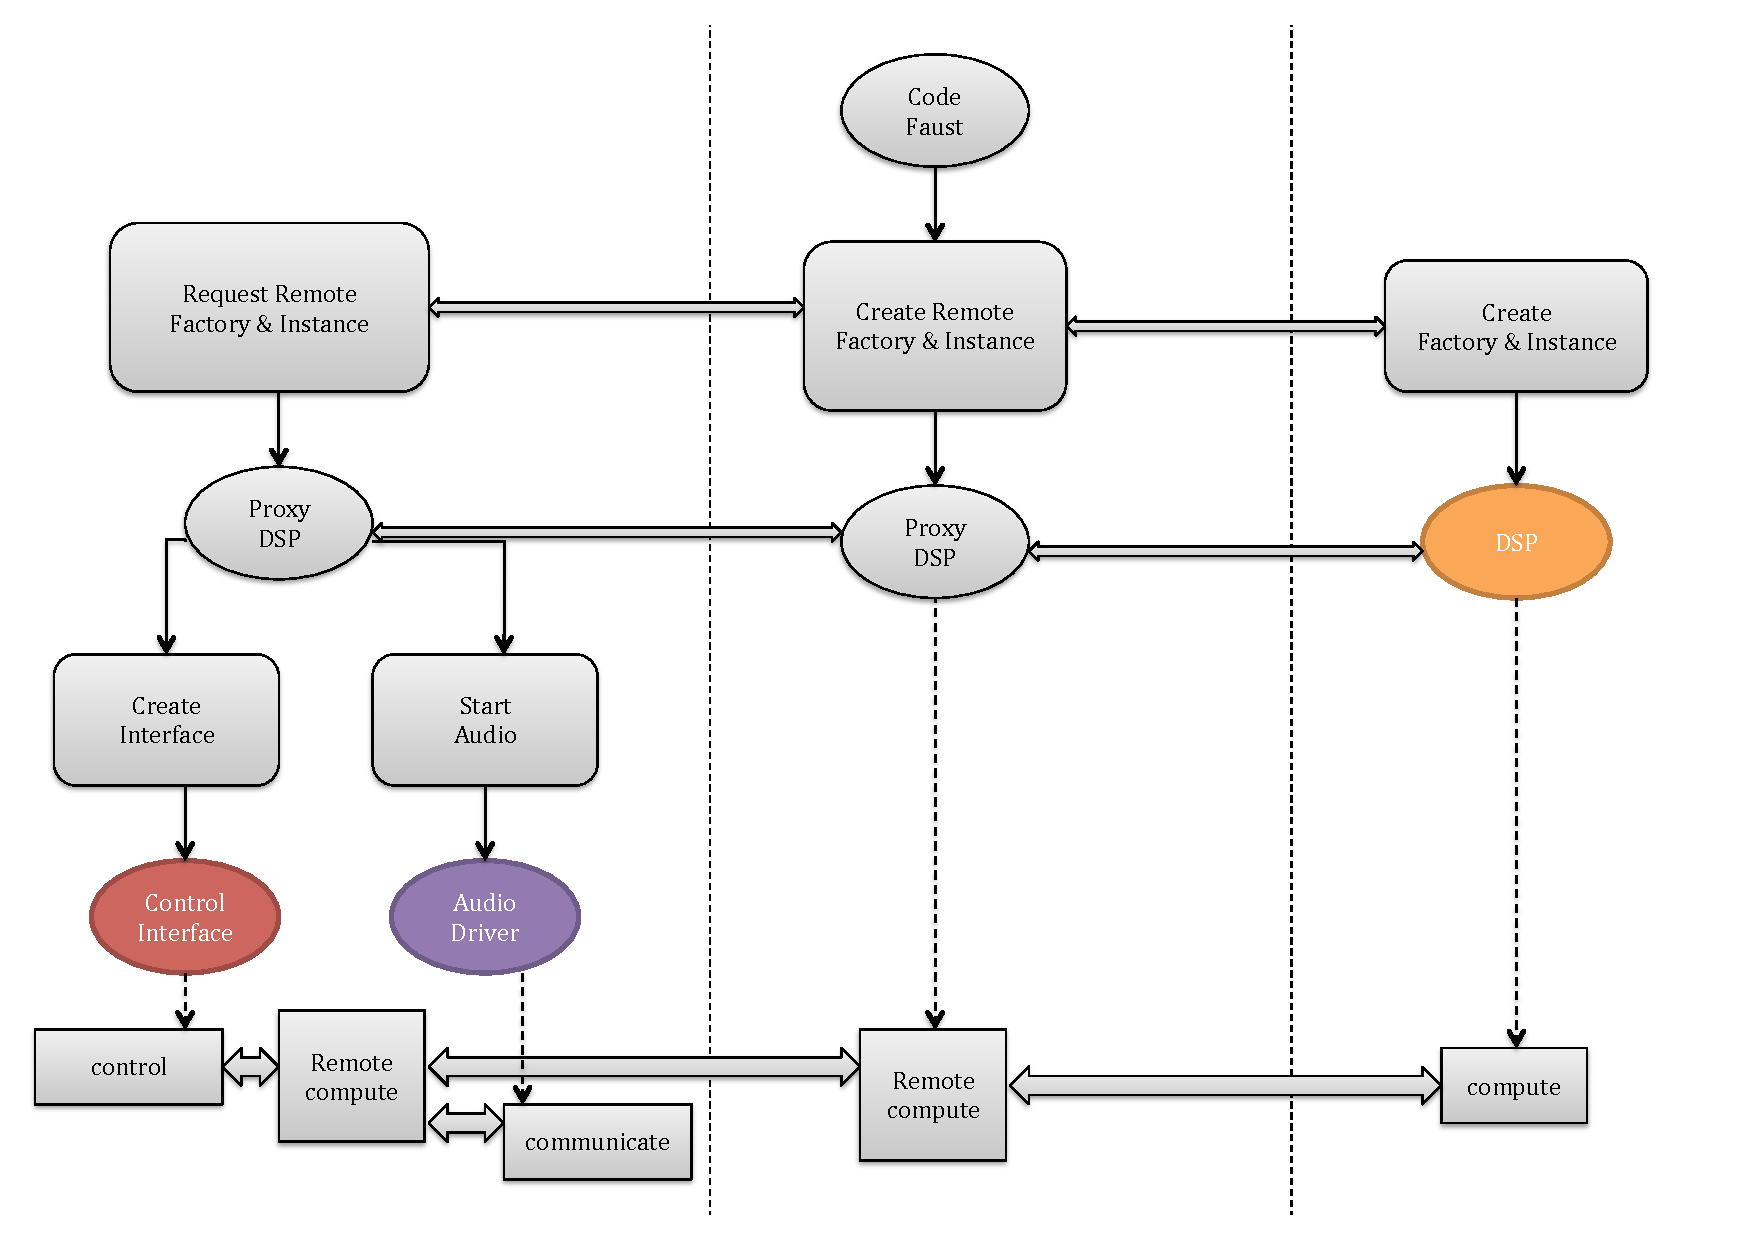
\includegraphics[width=0.9\columnwidth]{images/CCC9}
\end{minipage}
\caption{Creation of the Interface/DSP/Driver for a double remote processing situation}
\label{fig:CCC4}
\end{center}
\end{figure}

{\it Would it be possible to arrive in these situation (\ref{doubleprocessing} or \ref{synchronizedremote}) if the code was sent by the remote device or compiled on the other machine and discovered ? (See also \ref{constraints} for this kind of reflection)}

\newpage
\section{To keep in mind in each configuration}

\begin{itemize}
\item  Which interface(s) for the control ?
\item Where is the processing taking place ?
\item Where is the audio rendering taking place ?
\item Which network protocol(s) are used ?
\item Who has the Faust code in the first place and what chain of compilation is followed ?
\item What happen when the original code is modified (sync or not)?
\item What happens when one of the component is deleted ?
\item What happens when one the connection is lost ?
\end{itemize}

An example of interaction scenario in FaustLive for the imaginary \ref{synchronizedremote} scenario.

\begin{figure}[!h]
\begin{center}
\begin{minipage}[c]{\linewidth}
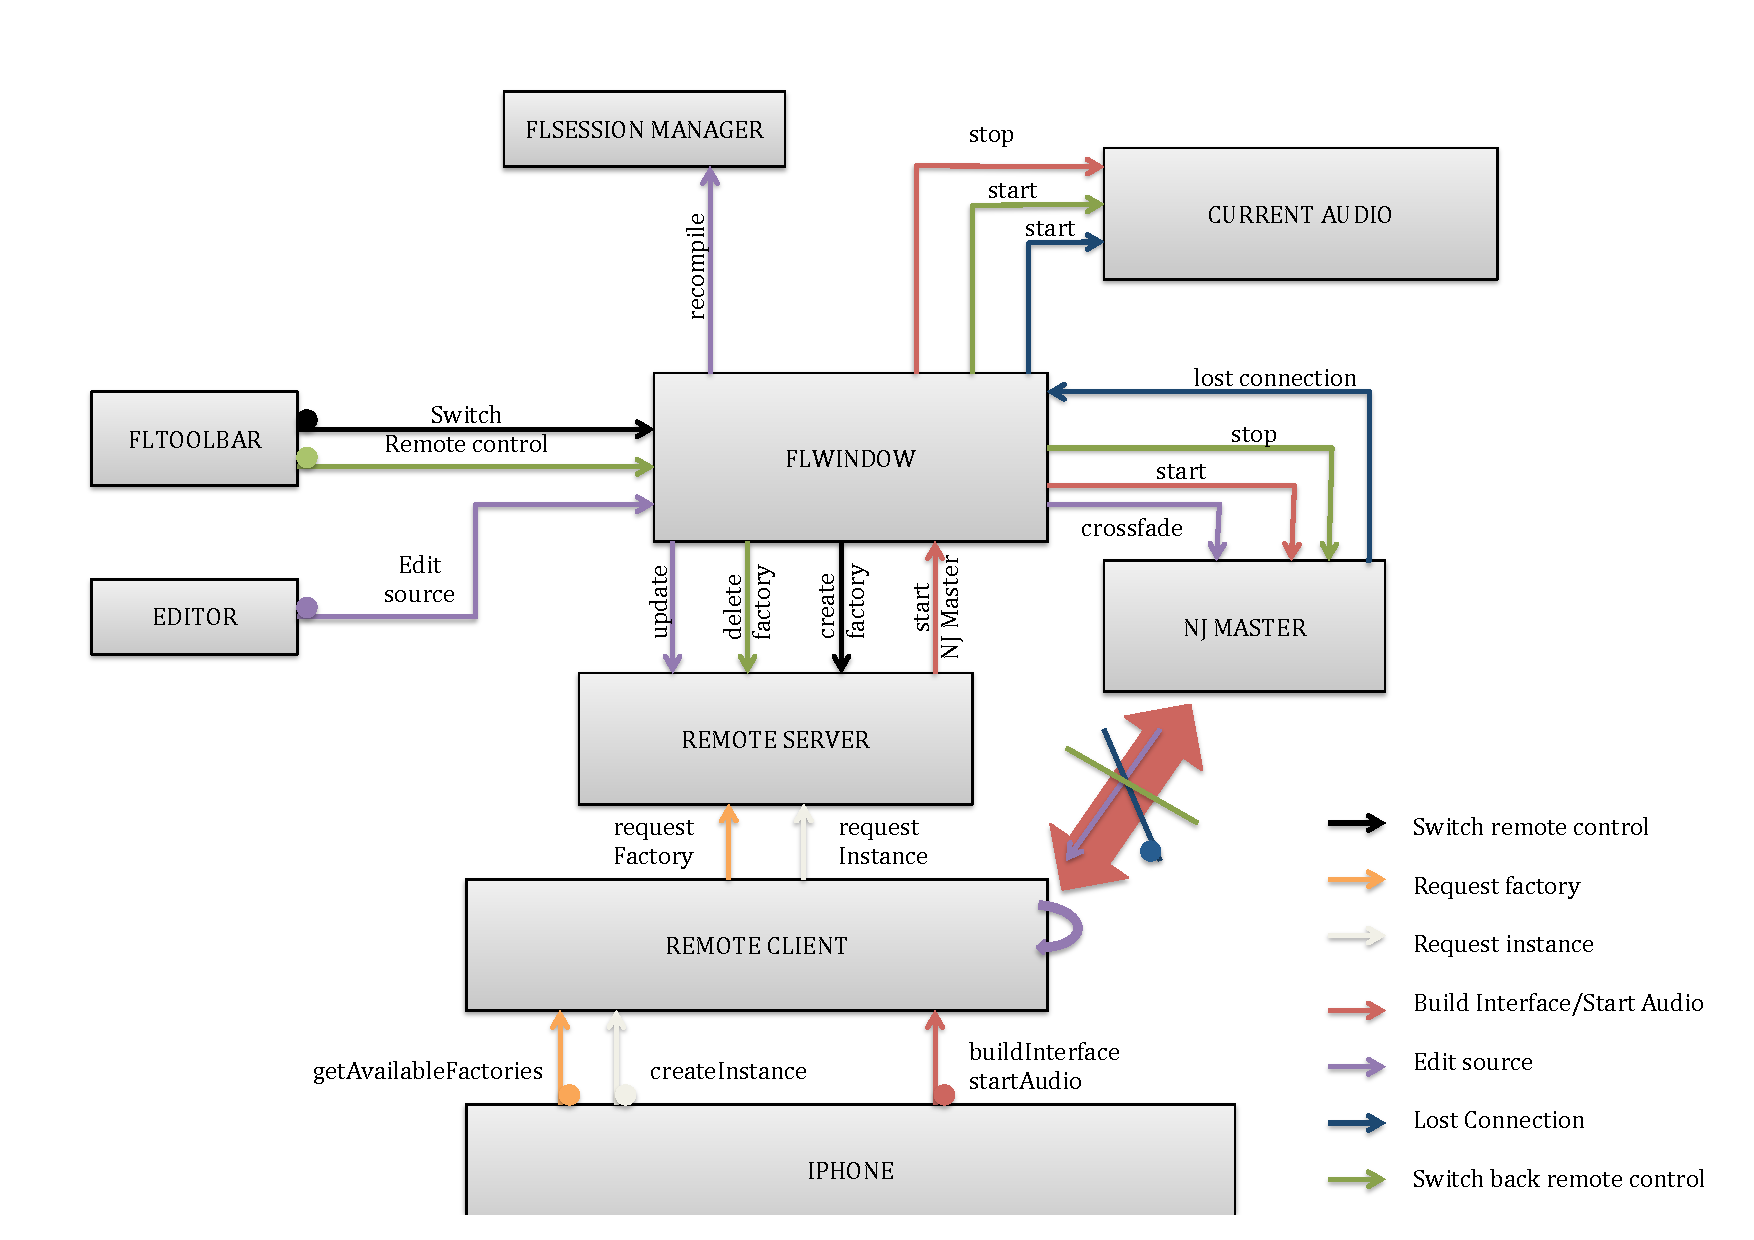
\includegraphics[width=0.9\columnwidth]{images/RemoteControl.pdf}
\end{minipage}
\caption{Class interactions in the synchronized remote processing scenario}
\label{fig:remotecontrolInteractions}
\end{center}
\end{figure}

\section{Attempts to checkout in FaustLive}

Some attempts have be added to FaustLive but never finished. See
\begin{itemize}
\item FLRemoteDSPScanner (and its use in FLApp)
\item FLRemoteServer (and its use in FLWindow)
\item FLInterfaceManager : it is trying to handle the synchronization of all the interface that right now is not very usefull because handle by the QT interface but when there is no QT interface who handles it ? (-->FLInterfaceManager)
\end{itemize}
\section{Conclusion}

It would be great to restructure the implementation of the web services that have very static implementations for exemple:
FLHTTPServer has its own "Post" function and its lot of html files to compose with. \\
Every HTTP Interface has its own logic \\
etc \\

Having a unique "POST" function would be an advance !

\end{document}




